% Options for packages loaded elsewhere
\PassOptionsToPackage{unicode}{hyperref}
\PassOptionsToPackage{hyphens}{url}
%
\documentclass[
]{article}
\title{Case Study 1}
\author{}
\date{\vspace{-2.5em}}

\usepackage{amsmath,amssymb}
\usepackage{lmodern}
\usepackage{iftex}
\ifPDFTeX
  \usepackage[T1]{fontenc}
  \usepackage[utf8]{inputenc}
  \usepackage{textcomp} % provide euro and other symbols
\else % if luatex or xetex
  \usepackage{unicode-math}
  \defaultfontfeatures{Scale=MatchLowercase}
  \defaultfontfeatures[\rmfamily]{Ligatures=TeX,Scale=1}
\fi
% Use upquote if available, for straight quotes in verbatim environments
\IfFileExists{upquote.sty}{\usepackage{upquote}}{}
\IfFileExists{microtype.sty}{% use microtype if available
  \usepackage[]{microtype}
  \UseMicrotypeSet[protrusion]{basicmath} % disable protrusion for tt fonts
}{}
\makeatletter
\@ifundefined{KOMAClassName}{% if non-KOMA class
  \IfFileExists{parskip.sty}{%
    \usepackage{parskip}
  }{% else
    \setlength{\parindent}{0pt}
    \setlength{\parskip}{6pt plus 2pt minus 1pt}}
}{% if KOMA class
  \KOMAoptions{parskip=half}}
\makeatother
\usepackage{xcolor}
\IfFileExists{xurl.sty}{\usepackage{xurl}}{} % add URL line breaks if available
\IfFileExists{bookmark.sty}{\usepackage{bookmark}}{\usepackage{hyperref}}
\hypersetup{
  pdftitle={Case Study 1},
  hidelinks,
  pdfcreator={LaTeX via pandoc}}
\urlstyle{same} % disable monospaced font for URLs
\usepackage[margin=1in]{geometry}
\usepackage{color}
\usepackage{fancyvrb}
\newcommand{\VerbBar}{|}
\newcommand{\VERB}{\Verb[commandchars=\\\{\}]}
\DefineVerbatimEnvironment{Highlighting}{Verbatim}{commandchars=\\\{\}}
% Add ',fontsize=\small' for more characters per line
\usepackage{framed}
\definecolor{shadecolor}{RGB}{248,248,248}
\newenvironment{Shaded}{\begin{snugshade}}{\end{snugshade}}
\newcommand{\AlertTok}[1]{\textcolor[rgb]{0.94,0.16,0.16}{#1}}
\newcommand{\AnnotationTok}[1]{\textcolor[rgb]{0.56,0.35,0.01}{\textbf{\textit{#1}}}}
\newcommand{\AttributeTok}[1]{\textcolor[rgb]{0.77,0.63,0.00}{#1}}
\newcommand{\BaseNTok}[1]{\textcolor[rgb]{0.00,0.00,0.81}{#1}}
\newcommand{\BuiltInTok}[1]{#1}
\newcommand{\CharTok}[1]{\textcolor[rgb]{0.31,0.60,0.02}{#1}}
\newcommand{\CommentTok}[1]{\textcolor[rgb]{0.56,0.35,0.01}{\textit{#1}}}
\newcommand{\CommentVarTok}[1]{\textcolor[rgb]{0.56,0.35,0.01}{\textbf{\textit{#1}}}}
\newcommand{\ConstantTok}[1]{\textcolor[rgb]{0.00,0.00,0.00}{#1}}
\newcommand{\ControlFlowTok}[1]{\textcolor[rgb]{0.13,0.29,0.53}{\textbf{#1}}}
\newcommand{\DataTypeTok}[1]{\textcolor[rgb]{0.13,0.29,0.53}{#1}}
\newcommand{\DecValTok}[1]{\textcolor[rgb]{0.00,0.00,0.81}{#1}}
\newcommand{\DocumentationTok}[1]{\textcolor[rgb]{0.56,0.35,0.01}{\textbf{\textit{#1}}}}
\newcommand{\ErrorTok}[1]{\textcolor[rgb]{0.64,0.00,0.00}{\textbf{#1}}}
\newcommand{\ExtensionTok}[1]{#1}
\newcommand{\FloatTok}[1]{\textcolor[rgb]{0.00,0.00,0.81}{#1}}
\newcommand{\FunctionTok}[1]{\textcolor[rgb]{0.00,0.00,0.00}{#1}}
\newcommand{\ImportTok}[1]{#1}
\newcommand{\InformationTok}[1]{\textcolor[rgb]{0.56,0.35,0.01}{\textbf{\textit{#1}}}}
\newcommand{\KeywordTok}[1]{\textcolor[rgb]{0.13,0.29,0.53}{\textbf{#1}}}
\newcommand{\NormalTok}[1]{#1}
\newcommand{\OperatorTok}[1]{\textcolor[rgb]{0.81,0.36,0.00}{\textbf{#1}}}
\newcommand{\OtherTok}[1]{\textcolor[rgb]{0.56,0.35,0.01}{#1}}
\newcommand{\PreprocessorTok}[1]{\textcolor[rgb]{0.56,0.35,0.01}{\textit{#1}}}
\newcommand{\RegionMarkerTok}[1]{#1}
\newcommand{\SpecialCharTok}[1]{\textcolor[rgb]{0.00,0.00,0.00}{#1}}
\newcommand{\SpecialStringTok}[1]{\textcolor[rgb]{0.31,0.60,0.02}{#1}}
\newcommand{\StringTok}[1]{\textcolor[rgb]{0.31,0.60,0.02}{#1}}
\newcommand{\VariableTok}[1]{\textcolor[rgb]{0.00,0.00,0.00}{#1}}
\newcommand{\VerbatimStringTok}[1]{\textcolor[rgb]{0.31,0.60,0.02}{#1}}
\newcommand{\WarningTok}[1]{\textcolor[rgb]{0.56,0.35,0.01}{\textbf{\textit{#1}}}}
\usepackage{graphicx}
\makeatletter
\def\maxwidth{\ifdim\Gin@nat@width>\linewidth\linewidth\else\Gin@nat@width\fi}
\def\maxheight{\ifdim\Gin@nat@height>\textheight\textheight\else\Gin@nat@height\fi}
\makeatother
% Scale images if necessary, so that they will not overflow the page
% margins by default, and it is still possible to overwrite the defaults
% using explicit options in \includegraphics[width, height, ...]{}
\setkeys{Gin}{width=\maxwidth,height=\maxheight,keepaspectratio}
% Set default figure placement to htbp
\makeatletter
\def\fps@figure{htbp}
\makeatother
\setlength{\emergencystretch}{3em} % prevent overfull lines
\providecommand{\tightlist}{%
  \setlength{\itemsep}{0pt}\setlength{\parskip}{0pt}}
\setcounter{secnumdepth}{-\maxdimen} % remove section numbering
\ifLuaTeX
  \usepackage{selnolig}  % disable illegal ligatures
\fi

\begin{document}
\maketitle

By Roslyn Smith, David George and Varun Gopal

This presentation investigates a few trends found in the Beers and
Breweries dataset. We reviewed trends across states in the U.S as well
as a deep dive on both ABV and IBU values. We also explored how ABV and
IBU can predict whether or not a beer is an IPA or an Ale.

Importing packages

\begin{Shaded}
\begin{Highlighting}[]
\CommentTok{\#Libraries}
\FunctionTok{library}\NormalTok{(tidyverse)}
\FunctionTok{library}\NormalTok{(caret)}
\FunctionTok{library}\NormalTok{(class)}
\FunctionTok{library}\NormalTok{(e1071)}
\FunctionTok{library}\NormalTok{(maps)}
\FunctionTok{library}\NormalTok{(mapproj)}
\FunctionTok{library}\NormalTok{(plotly)}
\FunctionTok{library}\NormalTok{(data.table)}
\FunctionTok{library}\NormalTok{(formattable)}
\FunctionTok{library}\NormalTok{(tidyr)}
\FunctionTok{library}\NormalTok{(dplyr)}
\end{Highlighting}
\end{Shaded}

Importing datasets

\begin{Shaded}
\begin{Highlighting}[]
\NormalTok{beers}\OtherTok{=}\FunctionTok{read.csv}\NormalTok{(}\StringTok{"Beers.csv"}\NormalTok{)}
\NormalTok{breweries}\OtherTok{=}\FunctionTok{read.csv}\NormalTok{(}\StringTok{"Breweries.csv"}\NormalTok{)}
\end{Highlighting}
\end{Shaded}

Question 3: Filter out NAs in beers

\begin{Shaded}
\begin{Highlighting}[]
\CommentTok{\#Filter out NAs in beers}
\NormalTok{beersclean}\OtherTok{=}\NormalTok{beers}\SpecialCharTok{\%\textgreater{}\%}\FunctionTok{filter}\NormalTok{(}\SpecialCharTok{!}\NormalTok{(}\FunctionTok{is.na}\NormalTok{(IBU)}\SpecialCharTok{|}\FunctionTok{is.na}\NormalTok{(ABV)))}
\NormalTok{ABVclean}\OtherTok{=}\NormalTok{beers}\SpecialCharTok{\%\textgreater{}\%}\FunctionTok{filter}\NormalTok{(}\SpecialCharTok{!}\FunctionTok{is.na}\NormalTok{(ABV))}
\NormalTok{IBUclean}\OtherTok{=}\NormalTok{beers}\SpecialCharTok{\%\textgreater{}\%}\FunctionTok{filter}\NormalTok{(}\SpecialCharTok{!}\FunctionTok{is.na}\NormalTok{(IBU))}
\end{Highlighting}
\end{Shaded}

In general, we decided to delete the entire row if an IBU or an ABV was
missing. However, there are some questions in which we only filtered out
missing ABV values when investigating only ABV values so that we could
keep more data. The same concept applied when investigating only IBU
values.

Question 1: Find how many breweries there are per state

\begin{Shaded}
\begin{Highlighting}[]
\CommentTok{\#Find how many breweries there are per state}
\CommentTok{\# Grouped Breweries by volume}
\NormalTok{breweriesclean }\OtherTok{=}\NormalTok{ breweries}\SpecialCharTok{\%\textgreater{}\%}\FunctionTok{group\_by}\NormalTok{(State)}\SpecialCharTok{\%\textgreater{}\%}
  \FunctionTok{summarize}\NormalTok{(}\AttributeTok{count=}\FunctionTok{n}\NormalTok{())}

\NormalTok{breweriessummary }\OtherTok{=}\NormalTok{ breweriesclean}\SpecialCharTok{\%\textgreater{}\%} 
  \FunctionTok{mutate}\NormalTok{(}\AttributeTok{Group =} \FunctionTok{case\_when}\NormalTok{(}
    \FunctionTok{between}\NormalTok{ (count,}\DecValTok{1}\NormalTok{,}\DecValTok{2}\NormalTok{)}\SpecialCharTok{\textasciitilde{}}\StringTok{"1 to 2 Breweries"}\NormalTok{,}
\NormalTok{    count }\SpecialCharTok{==}\DecValTok{3} \SpecialCharTok{\textasciitilde{}}\StringTok{"3 Breweries"}\NormalTok{,}
\NormalTok{    count }\SpecialCharTok{==}\DecValTok{4} \SpecialCharTok{\textasciitilde{}}\StringTok{"4 Breweries"}\NormalTok{,}
    \FunctionTok{between}\NormalTok{ (count,}\DecValTok{5}\NormalTok{,}\DecValTok{6}\NormalTok{)}\SpecialCharTok{\textasciitilde{}}\StringTok{"5 to 6 Breweries"}\NormalTok{,}
    \FunctionTok{between}\NormalTok{ (count,}\DecValTok{7}\NormalTok{,}\DecValTok{9}\NormalTok{)}\SpecialCharTok{\textasciitilde{}}\StringTok{"7 to 9 Breweries"}\NormalTok{,}
    \FunctionTok{between}\NormalTok{ (count,}\DecValTok{10}\NormalTok{,}\DecValTok{19}\NormalTok{)}\SpecialCharTok{\textasciitilde{}}\StringTok{"10 to 19 Breweries"}\NormalTok{,}
    \FunctionTok{between}\NormalTok{ (count,}\DecValTok{20}\NormalTok{,}\DecValTok{29}\NormalTok{)}\SpecialCharTok{\textasciitilde{}}\StringTok{"20 to 29 Breweries"}\NormalTok{,}
    \FunctionTok{between}\NormalTok{ (count,}\DecValTok{30}\NormalTok{,}\DecValTok{50}\NormalTok{)}\SpecialCharTok{\textasciitilde{}}\StringTok{"30+ Breweries"}
\NormalTok{  ))}


\CommentTok{\#Barplot of Breweries in Each State.  Note: x=reorder, "{-}" before count orders decending, no "{-}" orders ascending}

\NormalTok{breweriessummary}\SpecialCharTok{\%\textgreater{}\%}
  \FunctionTok{ggplot}\NormalTok{(}\FunctionTok{aes}\NormalTok{(}\AttributeTok{x=}\FunctionTok{reorder}\NormalTok{(State, count),}\AttributeTok{y=}\NormalTok{count, }\AttributeTok{fill=}\NormalTok{Group))}\SpecialCharTok{+}
  \FunctionTok{geom\_bar}\NormalTok{(}\AttributeTok{stat=}\StringTok{\textquotesingle{}identity\textquotesingle{}}\NormalTok{, }\AttributeTok{color =} \StringTok{"grey46"}\NormalTok{)}\SpecialCharTok{+}
  \FunctionTok{geom\_text}\NormalTok{(}\FunctionTok{aes}\NormalTok{(}\AttributeTok{label  =}\NormalTok{ count), }\AttributeTok{vjust =} \SpecialCharTok{{-}}\FloatTok{0.5}\NormalTok{, }\AttributeTok{size =} \FloatTok{2.5}\NormalTok{, }\AttributeTok{color =} \StringTok{"black"}\NormalTok{)}\SpecialCharTok{+}
  \FunctionTok{ggtitle}\NormalTok{(}\StringTok{\textquotesingle{}Number of Breweries per State\textquotesingle{}}\NormalTok{)}\SpecialCharTok{+}
  \FunctionTok{xlab}\NormalTok{(}\StringTok{\textquotesingle{}State\textquotesingle{}}\NormalTok{)}\SpecialCharTok{+}
  \FunctionTok{ylab}\NormalTok{(}\StringTok{\textquotesingle{}Number of Breweries\textquotesingle{}}\NormalTok{)}\SpecialCharTok{+}
  \FunctionTok{scale\_fill\_manual}\NormalTok{(}\StringTok{"Group"}\NormalTok{,}\AttributeTok{values =} \FunctionTok{c}\NormalTok{(}\StringTok{"1 to 2 Breweries"} \OtherTok{=} \StringTok{"gray96"}
\NormalTok{                                       ,}\StringTok{"3 Breweries"} \OtherTok{=} \StringTok{"seashell3"}
\NormalTok{                                       ,}\StringTok{"4 Breweries"} \OtherTok{=} \StringTok{"lightsteelblue"}
\NormalTok{                                       ,}\StringTok{"5 to 6 Breweries"}  \OtherTok{=} \StringTok{"lightskyblue1"}
\NormalTok{                                       ,}\StringTok{"7 to 9 Breweries"} \OtherTok{=} \StringTok{"deepskyblue"}
\NormalTok{                                       ,}\StringTok{"10 to 19 Breweries"} \OtherTok{=} \StringTok{"dodgerblue2"}
\NormalTok{                                       ,}\StringTok{"20 to 29 Breweries"} \OtherTok{=} \StringTok{"blue3"}
\NormalTok{                                       ,}\StringTok{"30+ Breweries"} \OtherTok{=} \StringTok{"midnightblue"}\NormalTok{) )}\SpecialCharTok{+}
  \FunctionTok{theme}\NormalTok{(}\AttributeTok{legend.position =} \StringTok{"bottom"}\NormalTok{,}
        \AttributeTok{legend.text =} \FunctionTok{element\_text}\NormalTok{(}\AttributeTok{size=}\DecValTok{7}\NormalTok{),}
        \AttributeTok{legend.title =} \FunctionTok{element\_blank}\NormalTok{(),}
        \AttributeTok{axis.text.y =} \FunctionTok{element\_blank}\NormalTok{(),}
        \AttributeTok{axis.title.y =} \FunctionTok{element\_blank}\NormalTok{(),}
        \AttributeTok{axis.ticks.y =} \FunctionTok{element\_blank}\NormalTok{(),}
        \AttributeTok{title =} \FunctionTok{element\_text}\NormalTok{(}\AttributeTok{face=}\StringTok{"bold"}\NormalTok{, }\AttributeTok{color =} \StringTok{"red3"}\NormalTok{, }\AttributeTok{size =} \DecValTok{8}\NormalTok{),}
        \AttributeTok{axis.title.x =} \FunctionTok{element\_text}\NormalTok{(}\AttributeTok{face=}\StringTok{"bold"}\NormalTok{, }\AttributeTok{color =} \StringTok{"dodgerblue3"}\NormalTok{, }\AttributeTok{size =} \DecValTok{9}\NormalTok{),}
        \AttributeTok{axis.text.x =} \FunctionTok{element\_text}\NormalTok{(}\AttributeTok{size =} \DecValTok{7}\NormalTok{))}\SpecialCharTok{+}
  \FunctionTok{scale\_y\_continuous}\NormalTok{(}\AttributeTok{minor\_breaks =} \FunctionTok{seq}\NormalTok{(}\DecValTok{0}\NormalTok{,}\DecValTok{50}\NormalTok{,}\DecValTok{10}\NormalTok{),}\AttributeTok{breaks=}\FunctionTok{seq}\NormalTok{(}\DecValTok{0}\NormalTok{,}\DecValTok{50}\NormalTok{,}\DecValTok{10}\NormalTok{))}
\end{Highlighting}
\end{Shaded}

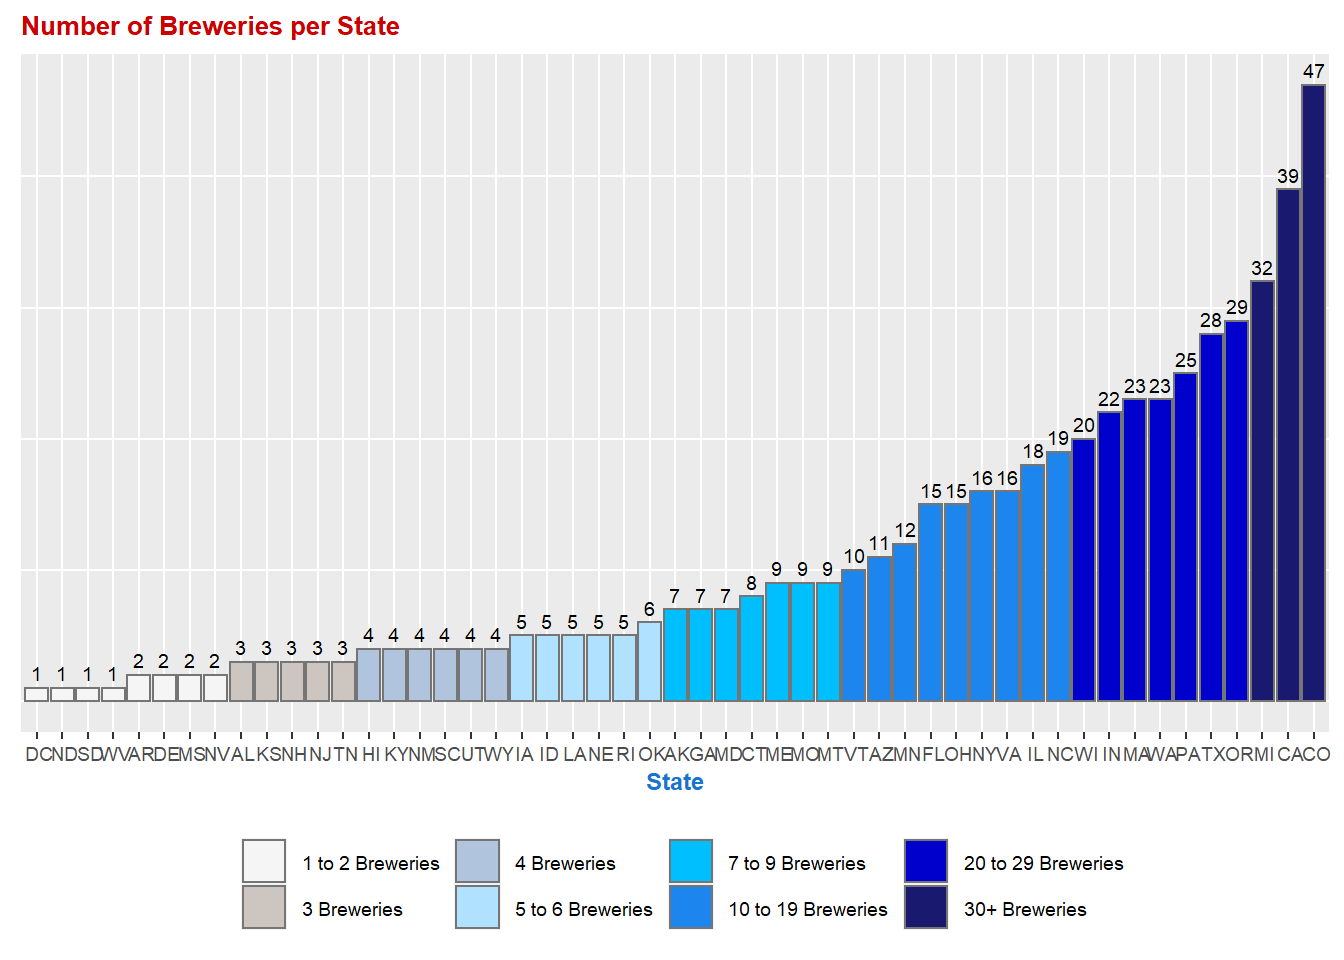
\includegraphics{Case-Study-Final_files/figure-latex/unnamed-chunk-4-1.pdf}

\begin{Shaded}
\begin{Highlighting}[]
\CommentTok{\#Create Heat Map }
\NormalTok{FiftyStates}\OtherTok{=}\FunctionTok{data.frame}\NormalTok{(}\AttributeTok{State=}\NormalTok{state.abb,}\AttributeTok{Name=}\NormalTok{state.name) }\CommentTok{\#Create and Name columns of DF}
\NormalTok{brewstates}\OtherTok{=}\NormalTok{breweries}\SpecialCharTok{\%\textgreater{}\%}\FunctionTok{group\_by}\NormalTok{(State)}\SpecialCharTok{\%\textgreater{}\%}
  \FunctionTok{summarize}\NormalTok{(}\AttributeTok{count=}\FunctionTok{n}\NormalTok{())}
\NormalTok{brewstates}\OtherTok{=}\FunctionTok{data.frame}\NormalTok{(breweriessummary)}
\ControlFlowTok{for}\NormalTok{ (i }\ControlFlowTok{in} \DecValTok{1}\SpecialCharTok{:}\FunctionTok{dim}\NormalTok{(brewstates)[}\DecValTok{1}\NormalTok{])\{}\CommentTok{\#Make sure the string values of FiftyStates and brewstates match for the upcoming merge}
\NormalTok{  brewstates}\SpecialCharTok{$}\NormalTok{State[i]}\OtherTok{=}\FunctionTok{str\_extract}\NormalTok{(brewstates}\SpecialCharTok{$}\NormalTok{State[i],}\StringTok{"}\SpecialCharTok{\textbackslash{}\textbackslash{}}\StringTok{b[A{-}Za{-}z]+}\SpecialCharTok{\textbackslash{}\textbackslash{}}\StringTok{b"}\NormalTok{)}
\NormalTok{\}}
\NormalTok{brewstates}\OtherTok{=}\FunctionTok{merge}\NormalTok{(brewstates,FiftyStates,}\StringTok{\textquotesingle{}State\textquotesingle{}}\NormalTok{,}\AttributeTok{all.x=}\ConstantTok{TRUE}\NormalTok{)}
\NormalTok{brewmapdata}\OtherTok{=}\FunctionTok{data.frame}\NormalTok{(}\AttributeTok{region=}\FunctionTok{tolower}\NormalTok{(brewstates}\SpecialCharTok{$}\NormalTok{Name),}\AttributeTok{Breweries=}\NormalTok{brewstates}\SpecialCharTok{$}\NormalTok{count, }\AttributeTok{State=}\NormalTok{brewstates}\SpecialCharTok{$}\NormalTok{State, }\AttributeTok{Group=}\NormalTok{brewstates}\SpecialCharTok{$}\NormalTok{Group)}\CommentTok{\#Create mapdata with regions column}

\NormalTok{States}\OtherTok{=}\FunctionTok{map\_data}\NormalTok{(}\StringTok{\textquotesingle{}state\textquotesingle{}}\NormalTok{)}
\NormalTok{map.df}\OtherTok{=}\FunctionTok{merge}\NormalTok{(States,brewmapdata,}\StringTok{"region"}\NormalTok{,}\AttributeTok{all.x=}\NormalTok{T)}\CommentTok{\#Finalize Map Data}
\NormalTok{map.df}\OtherTok{=}\NormalTok{map.df[}\FunctionTok{order}\NormalTok{(map.df}\SpecialCharTok{$}\NormalTok{order),]}

\NormalTok{map.df}\SpecialCharTok{\%\textgreater{}\%}\FunctionTok{ggplot}\NormalTok{(}\FunctionTok{aes}\NormalTok{(}\AttributeTok{x=}\NormalTok{long,}\AttributeTok{y=}\NormalTok{lat,}\AttributeTok{group=}\NormalTok{group))}\SpecialCharTok{+}
  \FunctionTok{geom\_polygon}\NormalTok{(}\FunctionTok{aes}\NormalTok{(}\AttributeTok{fill=}\NormalTok{Group))}\SpecialCharTok{+}
  \FunctionTok{geom\_path}\NormalTok{(}\AttributeTok{color =} \StringTok{"grey46"}\NormalTok{)}\SpecialCharTok{+}
  \FunctionTok{theme\_void}\NormalTok{()}\SpecialCharTok{+}
  \FunctionTok{scale\_fill\_manual}\NormalTok{(}\StringTok{"Group"}\NormalTok{,}\AttributeTok{values =} \FunctionTok{c}\NormalTok{(}\StringTok{"1 to 2 Breweries"} \OtherTok{=} \StringTok{"gray96"}
\NormalTok{                                       ,}\StringTok{"3 Breweries"} \OtherTok{=} \StringTok{"seashell3"}
\NormalTok{                                       ,}\StringTok{"4 Breweries"} \OtherTok{=} \StringTok{"lightsteelblue"}
\NormalTok{                                       ,}\StringTok{"5 to 6 Breweries"}  \OtherTok{=} \StringTok{"lightskyblue1"}
\NormalTok{                                       ,}\StringTok{"7 to 9 Breweries"} \OtherTok{=} \StringTok{"deepskyblue"}
\NormalTok{                                       ,}\StringTok{"10 to 19 Breweries"} \OtherTok{=} \StringTok{"dodgerblue2"}
\NormalTok{                                       ,}\StringTok{"20 to 29 Breweries"} \OtherTok{=} \StringTok{"blue3"}
\NormalTok{                                       ,}\StringTok{"30+ Breweries"} \OtherTok{=} \StringTok{"midnightblue"}\NormalTok{))}\SpecialCharTok{+}
  \FunctionTok{theme}\NormalTok{(}\AttributeTok{legend.position =} \StringTok{"bottom"}\NormalTok{,}
        \AttributeTok{legend.text =} \FunctionTok{element\_text}\NormalTok{(}\AttributeTok{size=}\DecValTok{7}\NormalTok{),}
        \AttributeTok{legend.title =} \FunctionTok{element\_blank}\NormalTok{(),}
        \AttributeTok{title =} \FunctionTok{element\_text}\NormalTok{(}\AttributeTok{face=}\StringTok{"bold"}\NormalTok{, }\AttributeTok{color =} \StringTok{"red3"}\NormalTok{, }\AttributeTok{size =} \DecValTok{12}\NormalTok{),}
        \AttributeTok{axis.text =} \FunctionTok{element\_blank}\NormalTok{(),}
        \AttributeTok{axis.title =} \FunctionTok{element\_blank}\NormalTok{(),}
        \AttributeTok{axis.ticks =} \FunctionTok{element\_blank}\NormalTok{())}\SpecialCharTok{+}
  \FunctionTok{ggtitle}\NormalTok{(}\StringTok{\textquotesingle{}Breweries by State\textquotesingle{}}\NormalTok{)}
\end{Highlighting}
\end{Shaded}

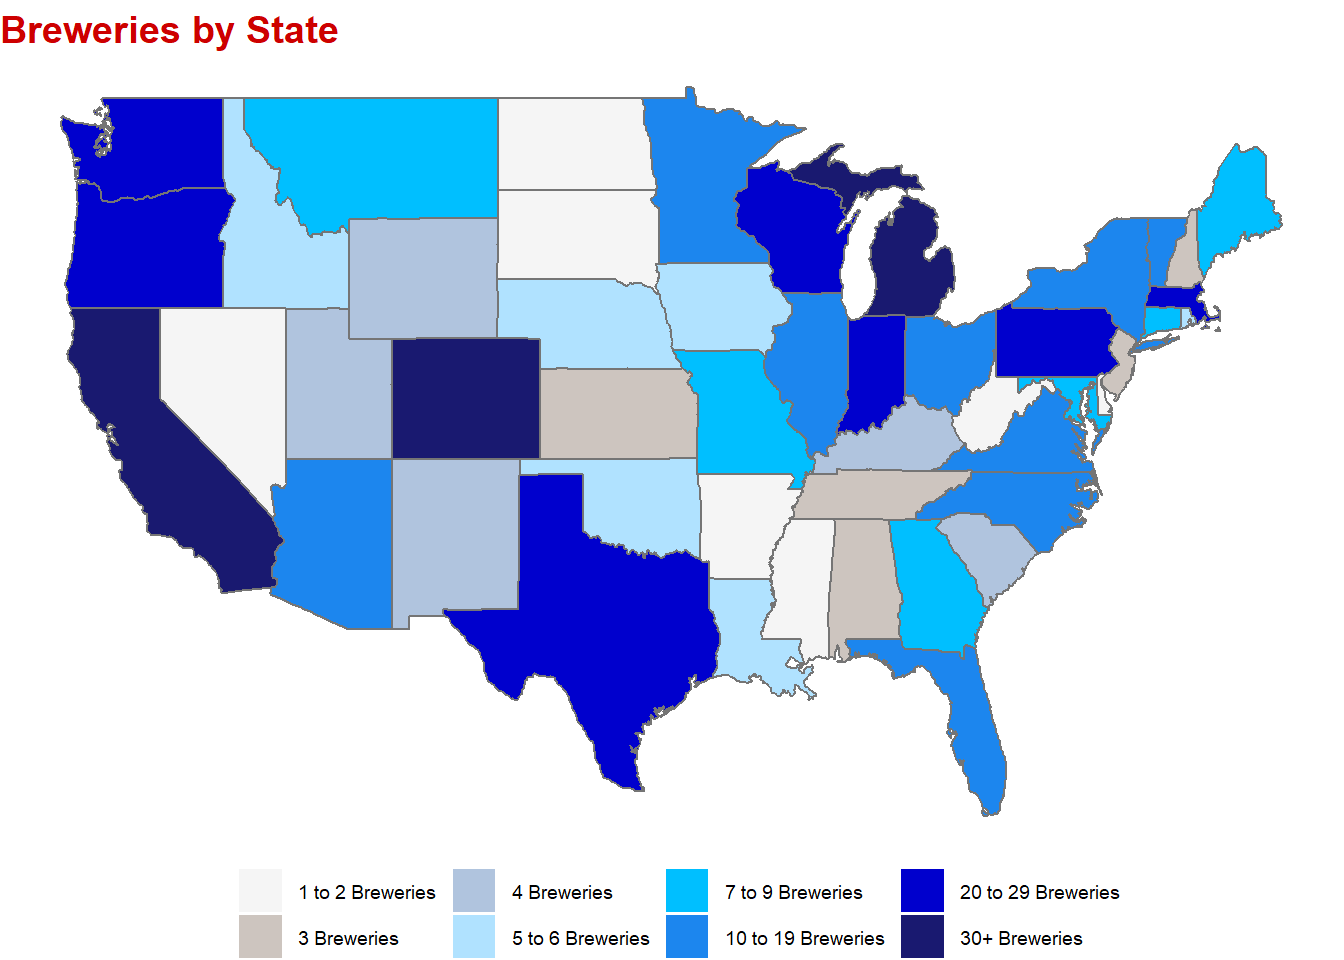
\includegraphics{Case-Study-Final_files/figure-latex/unnamed-chunk-4-2.pdf}

The barplot above shows the number of breweries for each state. There
are three states that have 30 or more breweries and those are Michigan,
California and Colorado. The heat map of the states also demonstrates
the same trend.

Question 2: Merge beer and breweries datasets

\begin{Shaded}
\begin{Highlighting}[]
\CommentTok{\#Merge beer and breweries}
\NormalTok{beersclean}\SpecialCharTok{$}\NormalTok{Brew\_ID}\OtherTok{=}\NormalTok{beersclean}\SpecialCharTok{$}\NormalTok{Brewery\_id}
\NormalTok{beerbreweries}\OtherTok{=}\FunctionTok{merge}\NormalTok{(beersclean,breweries,}\AttributeTok{by=}\StringTok{"Brew\_ID"}\NormalTok{,}\AttributeTok{all.x =} \ConstantTok{TRUE}\NormalTok{)}
\NormalTok{beerbreweries}\OtherTok{=}\NormalTok{beerbreweries}\SpecialCharTok{\%\textgreater{}\%}\FunctionTok{select}\NormalTok{(}\SpecialCharTok{!}\NormalTok{Brewery\_id)}

\CommentTok{\#Merge cleaned ABV data with breweries}
\NormalTok{ABVclean}\SpecialCharTok{$}\NormalTok{Brew\_ID}\OtherTok{=}\NormalTok{ABVclean}\SpecialCharTok{$}\NormalTok{Brewery\_id}
\NormalTok{ABVbreweries}\OtherTok{=}\FunctionTok{merge}\NormalTok{(ABVclean,breweries,}\AttributeTok{by=}\StringTok{"Brew\_ID"}\NormalTok{,}\AttributeTok{all.x =} \ConstantTok{TRUE}\NormalTok{)}
\NormalTok{ABVbreweries}\OtherTok{=}\NormalTok{ABVbreweries}\SpecialCharTok{\%\textgreater{}\%}\FunctionTok{select}\NormalTok{(}\SpecialCharTok{!}\NormalTok{Brewery\_id)}

\CommentTok{\#Merge cleaned IBU data with breweries}
\NormalTok{IBUclean}\SpecialCharTok{$}\NormalTok{Brew\_ID}\OtherTok{=}\NormalTok{IBUclean}\SpecialCharTok{$}\NormalTok{Brewery\_id}
\NormalTok{IBUbreweries}\OtherTok{=}\FunctionTok{merge}\NormalTok{(IBUclean,breweries,}\AttributeTok{by=}\StringTok{"Brew\_ID"}\NormalTok{,}\AttributeTok{all.x =} \ConstantTok{TRUE}\NormalTok{)}
\NormalTok{IBUbreweries}\OtherTok{=}\NormalTok{IBUbreweries}\SpecialCharTok{\%\textgreater{}\%}\FunctionTok{select}\NormalTok{(}\SpecialCharTok{!}\NormalTok{Brewery\_id)}

\CommentTok{\#Print first 6 and last 6 observations}
\FunctionTok{head}\NormalTok{(beerbreweries)}
\end{Highlighting}
\end{Shaded}

\begin{verbatim}
##   Brew_ID        Name.x Beer_ID   ABV IBU                               Style Ounces             Name.y        City State
## 1       1  Get Together    2692 0.045  50                        American IPA     16 NorthGate Brewing  Minneapolis    MN
## 2       1 Maggie's Leap    2691 0.049  26                  Milk / Sweet Stout     16 NorthGate Brewing  Minneapolis    MN
## 3       1    Wall's End    2690 0.048  19                   English Brown Ale     16 NorthGate Brewing  Minneapolis    MN
## 4       1       Pumpion    2689 0.060  38                         Pumpkin Ale     16 NorthGate Brewing  Minneapolis    MN
## 5       1    Stronghold    2688 0.060  25                     American Porter     16 NorthGate Brewing  Minneapolis    MN
## 6       1   Parapet ESB    2687 0.056  47 Extra Special / Strong Bitter (ESB)     16 NorthGate Brewing  Minneapolis    MN
\end{verbatim}

\begin{Shaded}
\begin{Highlighting}[]
\FunctionTok{tail}\NormalTok{(beerbreweries)}
\end{Highlighting}
\end{Shaded}

\begin{verbatim}
##      Brew_ID                           Name.x Beer_ID   ABV IBU                 Style Ounces                    Name.y      City State
## 1400     545        Pyramid Hefeweizen (2011)     399 0.052  18            Hefeweizen     12         Pyramid Breweries   Seattle    WA
## 1401     545        Haywire Hefeweizen (2010)      82 0.052  18            Hefeweizen     16         Pyramid Breweries   Seattle    WA
## 1402     546           Rumspringa Golden Bock     392 0.066  30 Maibock / Helles Bock     12 Lancaster Brewing Company Lancaster    PA
## 1403     546   Lancaster German Style Kölsch     195 0.048  28               Kölsch     12 Lancaster Brewing Company Lancaster    PA
## 1404     547 Common Sense Kentucky Common Ale     382 0.053  22    American Brown Ale     16   Upstate Brewing Company    Elmira    NY
## 1405     547                   Upstate I.P.W.     381 0.065  70          American IPA     12   Upstate Brewing Company    Elmira    NY
\end{verbatim}

We merged the beers and breweries datasets by brewery id and by using a
left join. We also merged the dataset containing non-NA ABV's and the
breweries dataset for investigating ABV values only. The same concept
applied when investigating only IBU values.

Question 4: Find median ABV and IBU per state

\begin{Shaded}
\begin{Highlighting}[]
\CommentTok{\#Find median ABV and IBU per state}
\FunctionTok{colnames}\NormalTok{(beerbreweries)[}\DecValTok{8}\NormalTok{]}\OtherTok{=}\StringTok{\textquotesingle{}Brewery\_Name\textquotesingle{}}
\FunctionTok{colnames}\NormalTok{(beerbreweries)[}\DecValTok{2}\NormalTok{]}\OtherTok{=}\StringTok{\textquotesingle{}Beer\_Name\textquotesingle{}}

\FunctionTok{colnames}\NormalTok{(ABVbreweries)[}\DecValTok{8}\NormalTok{]}\OtherTok{=}\StringTok{\textquotesingle{}Brewery\_Name\textquotesingle{}}
\FunctionTok{colnames}\NormalTok{(ABVbreweries)[}\DecValTok{2}\NormalTok{]}\OtherTok{=}\StringTok{\textquotesingle{}Beer\_Name\textquotesingle{}}

\FunctionTok{colnames}\NormalTok{(IBUbreweries)[}\DecValTok{8}\NormalTok{]}\OtherTok{=}\StringTok{\textquotesingle{}Brewery\_Name\textquotesingle{}}
\FunctionTok{colnames}\NormalTok{(IBUbreweries)[}\DecValTok{2}\NormalTok{]}\OtherTok{=}\StringTok{\textquotesingle{}Beer\_Name\textquotesingle{}}


\CommentTok{\#Gather median abv and ibu per each state}
\NormalTok{ABVIBUData}\OtherTok{=}\NormalTok{beerbreweries}\SpecialCharTok{\%\textgreater{}\%}\FunctionTok{group\_by}\NormalTok{(State)}\SpecialCharTok{\%\textgreater{}\%}\FunctionTok{summarize}\NormalTok{(}\AttributeTok{medianABV=}\FunctionTok{median}\NormalTok{(ABV),}\AttributeTok{medianIBU=}\FunctionTok{median}\NormalTok{(IBU),}\AttributeTok{count=}\FunctionTok{n}\NormalTok{())}
\NormalTok{ABVData}\OtherTok{=}\NormalTok{ABVbreweries}\SpecialCharTok{\%\textgreater{}\%}\FunctionTok{group\_by}\NormalTok{(State)}\SpecialCharTok{\%\textgreater{}\%}\FunctionTok{summarize}\NormalTok{(}\AttributeTok{medianABV=}\FunctionTok{median}\NormalTok{(ABV),}\AttributeTok{count=}\FunctionTok{n}\NormalTok{())}
\NormalTok{IBUData}\OtherTok{=}\NormalTok{IBUbreweries}\SpecialCharTok{\%\textgreater{}\%}\FunctionTok{group\_by}\NormalTok{(State)}\SpecialCharTok{\%\textgreater{}\%}\FunctionTok{summarize}\NormalTok{(}\AttributeTok{medianIBU=}\FunctionTok{median}\NormalTok{(IBU),}\AttributeTok{count=}\FunctionTok{n}\NormalTok{())}


\CommentTok{\#barplot ABV Updated}

\NormalTok{ABVData}\SpecialCharTok{\%\textgreater{}\%}
  \FunctionTok{ggplot}\NormalTok{(}\FunctionTok{aes}\NormalTok{(}\AttributeTok{x=}\FunctionTok{reorder}\NormalTok{(State,medianABV),}\AttributeTok{y=}\NormalTok{medianABV,}\AttributeTok{fill=}\NormalTok{medianABV))}\SpecialCharTok{+}
  \FunctionTok{geom\_bar}\NormalTok{(}\AttributeTok{stat=}\StringTok{\textquotesingle{}identity\textquotesingle{}}\NormalTok{, }\AttributeTok{color =} \StringTok{"grey46"}\NormalTok{)}\SpecialCharTok{+}
  \FunctionTok{geom\_text}\NormalTok{(}\FunctionTok{aes}\NormalTok{(}\AttributeTok{label  =}\NormalTok{ medianABV), }\AttributeTok{vjust =} \SpecialCharTok{{-}}\FloatTok{1.5}\NormalTok{, }\AttributeTok{size =} \FloatTok{2.2}\NormalTok{, }\AttributeTok{color =} \StringTok{"black"}\NormalTok{,}\AttributeTok{fontface =}  \StringTok{"bold"}\NormalTok{,}\AttributeTok{check\_overlap =} \ConstantTok{TRUE}\NormalTok{)}\SpecialCharTok{+}
  \FunctionTok{ylim}\NormalTok{(}\DecValTok{0}\NormalTok{,.}\DecValTok{073}\NormalTok{)}\SpecialCharTok{+}
  \FunctionTok{ggtitle}\NormalTok{(}\StringTok{\textquotesingle{}Median ABV by State\textquotesingle{}}\NormalTok{)}\SpecialCharTok{+}
  \FunctionTok{xlab}\NormalTok{(}\StringTok{\textquotesingle{}State\textquotesingle{}}\NormalTok{)}\SpecialCharTok{+}
  \FunctionTok{ylab}\NormalTok{(}\StringTok{\textquotesingle{}Median ABV\textquotesingle{}}\NormalTok{)}\SpecialCharTok{+}
  \FunctionTok{scale\_fill\_gradient2}\NormalTok{(}\AttributeTok{name=}\StringTok{\textquotesingle{}Median ABV\textquotesingle{}}\NormalTok{,}\AttributeTok{low =} \StringTok{"white"}\NormalTok{, }\AttributeTok{mid =} \StringTok{"steelblue1"}\NormalTok{, }\AttributeTok{high =} \StringTok{"midnightblue"}\NormalTok{,}\AttributeTok{midpoint =} \FloatTok{0.05}\NormalTok{, }\AttributeTok{limits =} \FunctionTok{c}\NormalTok{(}\FloatTok{0.03}\NormalTok{,}\FloatTok{0.07}\NormalTok{), }
                       \AttributeTok{breaks=}\FunctionTok{c}\NormalTok{(}\FloatTok{0.03}\NormalTok{,}\FloatTok{0.038}\NormalTok{,}\FloatTok{0.046}\NormalTok{,}\FloatTok{0.054}\NormalTok{,}\FloatTok{0.062}\NormalTok{,}\FloatTok{0.07}\NormalTok{), }\AttributeTok{na.value =} \StringTok{"grey50"}\NormalTok{)}\SpecialCharTok{+}
  \FunctionTok{theme}\NormalTok{(}\AttributeTok{legend.position =} \StringTok{"none"}\NormalTok{,}
        \AttributeTok{title =} \FunctionTok{element\_text}\NormalTok{(}\AttributeTok{face=}\StringTok{"bold"}\NormalTok{, }\AttributeTok{color =} \StringTok{"red3"}\NormalTok{, }\AttributeTok{size =} \DecValTok{12}\NormalTok{),}
        \AttributeTok{axis.text.y =} \FunctionTok{element\_blank}\NormalTok{(),}
        \AttributeTok{axis.title.y =} \FunctionTok{element\_blank}\NormalTok{(),}
        \AttributeTok{axis.ticks.y =} \FunctionTok{element\_blank}\NormalTok{(),}
        \AttributeTok{axis.text.x =} \FunctionTok{element\_text}\NormalTok{(}\AttributeTok{size =} \DecValTok{7}\NormalTok{),}
        \AttributeTok{axis.title.x =} \FunctionTok{element\_text}\NormalTok{(}\AttributeTok{face=}\StringTok{"bold"}\NormalTok{, }\AttributeTok{color =} \StringTok{"red3"}\NormalTok{, }\AttributeTok{size =} \DecValTok{9}\NormalTok{))}
\end{Highlighting}
\end{Shaded}

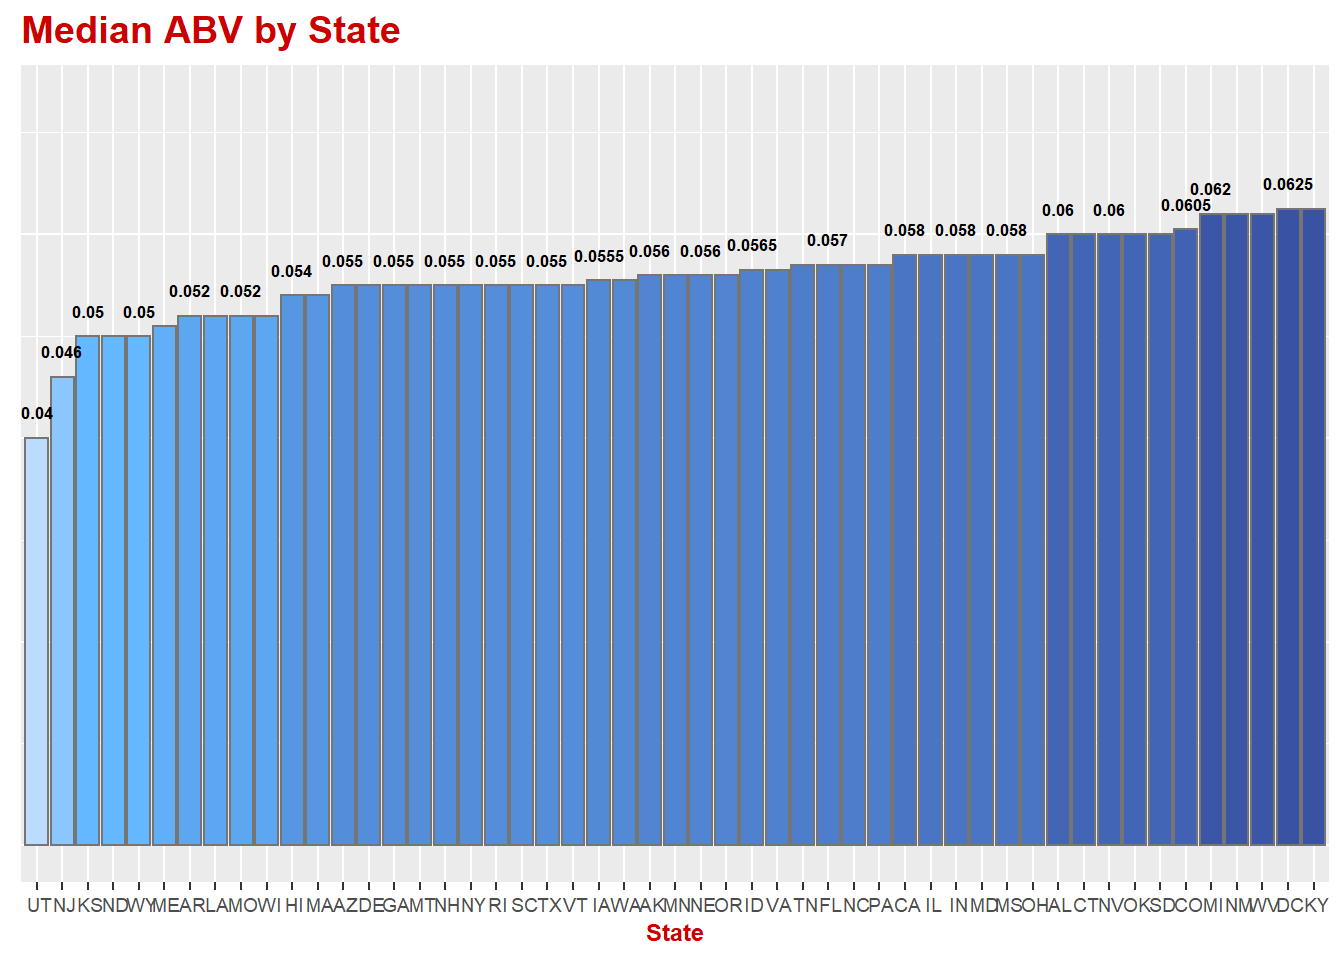
\includegraphics{Case-Study-Final_files/figure-latex/unnamed-chunk-6-1.pdf}

\begin{Shaded}
\begin{Highlighting}[]
\CommentTok{\#barplot IBU Updated}
\NormalTok{IBUData}\SpecialCharTok{\%\textgreater{}\%}\FunctionTok{ggplot}\NormalTok{(}\FunctionTok{aes}\NormalTok{(}\AttributeTok{x=}\FunctionTok{reorder}\NormalTok{(State,medianIBU),}\AttributeTok{y=}\NormalTok{medianIBU,}\AttributeTok{fill=}\NormalTok{medianIBU))}\SpecialCharTok{+}
  \FunctionTok{geom\_bar}\NormalTok{(}\AttributeTok{stat=}\StringTok{\textquotesingle{}identity\textquotesingle{}}\NormalTok{, }\AttributeTok{color =} \StringTok{"grey46"}\NormalTok{)}\SpecialCharTok{+}
  \FunctionTok{geom\_text}\NormalTok{(}\FunctionTok{aes}\NormalTok{(}\AttributeTok{label  =}\NormalTok{ medianIBU), }\AttributeTok{vjust =} \SpecialCharTok{{-}}\FloatTok{1.5}\NormalTok{, }\AttributeTok{size =} \FloatTok{2.3}\NormalTok{, }\AttributeTok{color =} \StringTok{"black"}\NormalTok{,}\AttributeTok{fontface =}  \StringTok{"bold"}\NormalTok{,}\AttributeTok{check\_overlap =} \ConstantTok{TRUE}\NormalTok{)}\SpecialCharTok{+}
  \FunctionTok{ylim}\NormalTok{(}\DecValTok{0}\NormalTok{,}\DecValTok{70}\NormalTok{)}\SpecialCharTok{+}
  \FunctionTok{ggtitle}\NormalTok{(}\StringTok{\textquotesingle{}Median IBU by State\textquotesingle{}}\NormalTok{)}\SpecialCharTok{+}
  \FunctionTok{xlab}\NormalTok{(}\StringTok{\textquotesingle{}State\textquotesingle{}}\NormalTok{)}\SpecialCharTok{+}
  \FunctionTok{ylab}\NormalTok{(}\StringTok{\textquotesingle{}Median IBU\textquotesingle{}}\NormalTok{)}\SpecialCharTok{+}
  \FunctionTok{scale\_fill\_gradient2}\NormalTok{(}\AttributeTok{name=}\StringTok{\textquotesingle{}Median IBU\textquotesingle{}}\NormalTok{,}\AttributeTok{low =} \StringTok{"white"}\NormalTok{, }\AttributeTok{mid =} \StringTok{"red"}\NormalTok{, }\AttributeTok{high =} \StringTok{"red4"}\NormalTok{, }
                       \AttributeTok{midpoint =} \DecValTok{40}\NormalTok{, }\AttributeTok{limits =} \FunctionTok{c}\NormalTok{(}\DecValTok{10}\NormalTok{,}\DecValTok{70}\NormalTok{), }
                       \AttributeTok{breaks=}\FunctionTok{c}\NormalTok{(}\DecValTok{10}\NormalTok{,}\DecValTok{22}\NormalTok{,}\DecValTok{34}\NormalTok{,}\DecValTok{46}\NormalTok{,}\DecValTok{58}\NormalTok{,}\DecValTok{70}\NormalTok{), }\AttributeTok{na.value =} \StringTok{"grey50"}\NormalTok{)}\SpecialCharTok{+}
  \FunctionTok{theme}\NormalTok{(}\AttributeTok{legend.position =} \StringTok{"none"}\NormalTok{,}
        \AttributeTok{title =} \FunctionTok{element\_text}\NormalTok{(}\AttributeTok{face=}\StringTok{"bold"}\NormalTok{, }\AttributeTok{color =} \StringTok{"midnightblue"}\NormalTok{, }\AttributeTok{size =} \DecValTok{12}\NormalTok{),}
        \AttributeTok{axis.text.y =} \FunctionTok{element\_blank}\NormalTok{(),}
        \AttributeTok{axis.title.y =} \FunctionTok{element\_blank}\NormalTok{(),}
        \AttributeTok{axis.ticks.y =} \FunctionTok{element\_blank}\NormalTok{(),}
        \AttributeTok{axis.title.x =} \FunctionTok{element\_text}\NormalTok{(}\AttributeTok{face=}\StringTok{"bold"}\NormalTok{, }\AttributeTok{color =} \StringTok{"midnightblue"}\NormalTok{, }\AttributeTok{size =} \DecValTok{9}\NormalTok{),}
        \AttributeTok{axis.text.x =} \FunctionTok{element\_text}\NormalTok{(}\AttributeTok{size =} \DecValTok{7}\NormalTok{))}
\end{Highlighting}
\end{Shaded}

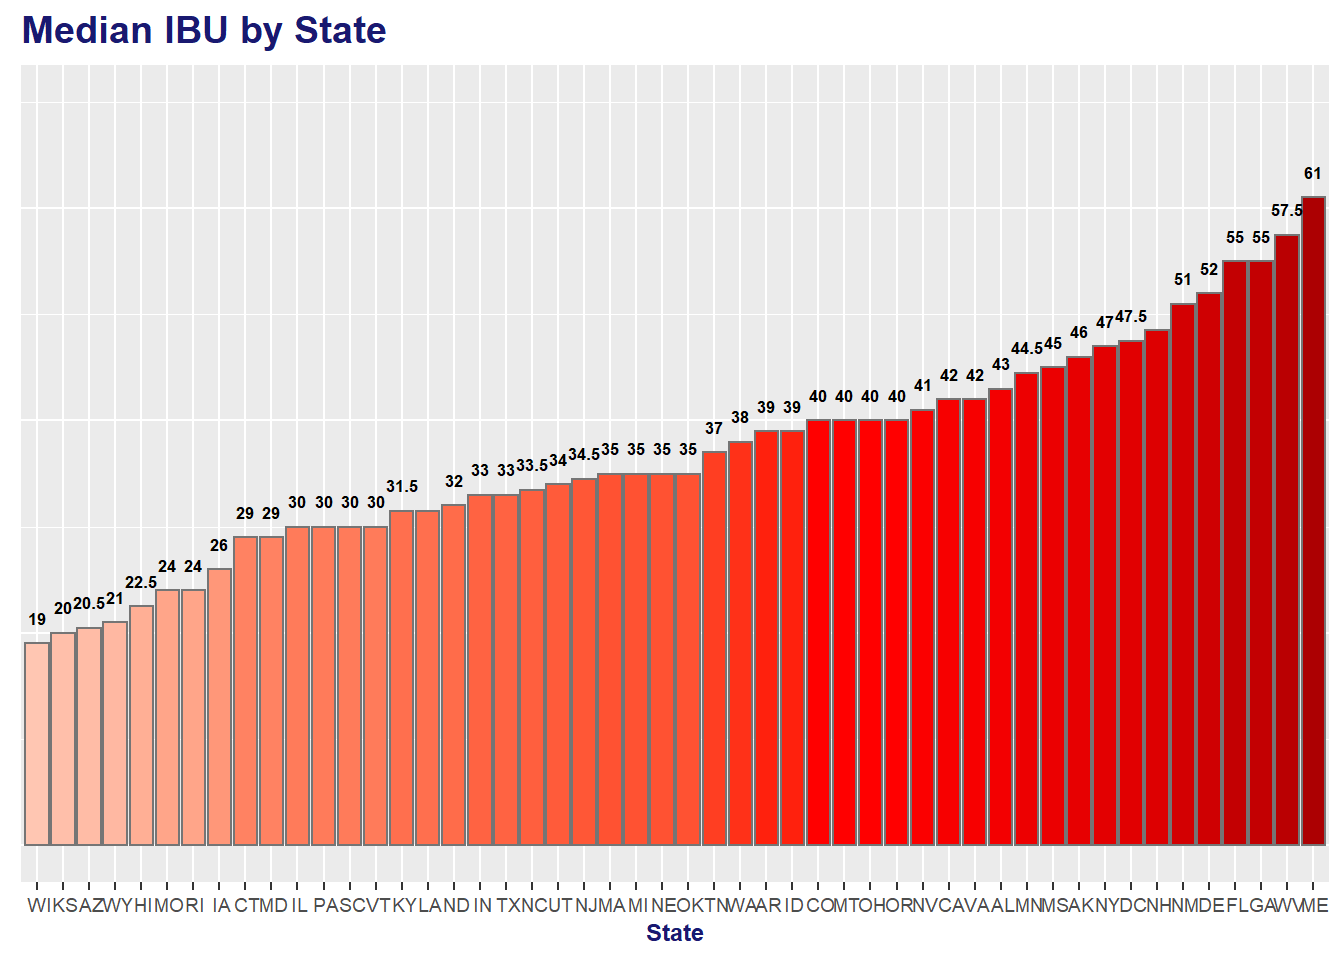
\includegraphics{Case-Study-Final_files/figure-latex/unnamed-chunk-6-2.pdf}

The bar charts of median ABV per state and the median IBU per state are
shown above. The two states with the highest median ABV were Kentucky
and Washington DC with 0.625. The state with the lowest median ABV was
Utah (0.04). The state with the highest median IBU was Maine (score of
61) whereas the state with the lowest median IBU was Wisconsin (19).

\begin{Shaded}
\begin{Highlighting}[]
\CommentTok{\#Find State w/ Max ABV and IBU when all NAs are deleted}
\NormalTok{ABVData}\SpecialCharTok{\%\textgreater{}\%}\FunctionTok{filter}\NormalTok{(medianABV}\SpecialCharTok{==}\FunctionTok{max}\NormalTok{(medianABV))}
\end{Highlighting}
\end{Shaded}

\begin{verbatim}
## # A tibble: 2 x 3
##   State medianABV count
##   <chr>     <dbl> <int>
## 1 " DC"    0.0625     8
## 2 " KY"    0.0625    20
\end{verbatim}

\begin{Shaded}
\begin{Highlighting}[]
\NormalTok{IBUData}\SpecialCharTok{\%\textgreater{}\%}\FunctionTok{filter}\NormalTok{(medianIBU}\SpecialCharTok{==}\FunctionTok{max}\NormalTok{(medianIBU))}
\end{Highlighting}
\end{Shaded}

\begin{verbatim}
## # A tibble: 1 x 3
##   State medianIBU count
##   <chr>     <dbl> <int>
## 1 " ME"        61     7
\end{verbatim}

\begin{Shaded}
\begin{Highlighting}[]
\NormalTok{ABVIBUData}\SpecialCharTok{\%\textgreater{}\%}\FunctionTok{filter}\NormalTok{(medianIBU}\SpecialCharTok{==}\FunctionTok{max}\NormalTok{(medianIBU))}
\end{Highlighting}
\end{Shaded}

\begin{verbatim}
## # A tibble: 1 x 4
##   State medianABV medianIBU count
##   <chr>     <dbl>     <dbl> <int>
## 1 " ME"     0.067        61     7
\end{verbatim}

\begin{Shaded}
\begin{Highlighting}[]
\NormalTok{HighABVIBU}\OtherTok{=}\NormalTok{ABVIBUData}\SpecialCharTok{\%\textgreater{}\%}\FunctionTok{filter}\NormalTok{(medianABV}\SpecialCharTok{==}\FunctionTok{max}\NormalTok{(medianABV))}



\CommentTok{\#Find State w/ Max ABV and IBU based on updated cleanup (separate for ABV and IBU)}
\NormalTok{HighABV}\OtherTok{=}\NormalTok{ABVData}\SpecialCharTok{\%\textgreater{}\%}\FunctionTok{filter}\NormalTok{(medianABV}\SpecialCharTok{==}\FunctionTok{max}\NormalTok{(medianABV))}



\NormalTok{HighIBU}\OtherTok{=}\NormalTok{IBUData}\SpecialCharTok{\%\textgreater{}\%}\FunctionTok{filter}\NormalTok{(medianIBU}\SpecialCharTok{==}\FunctionTok{max}\NormalTok{(medianIBU))}
\end{Highlighting}
\end{Shaded}

The first table shows that when accounting for all present ABV values,
KY and DC have the highest median ABV. In the second table, when
accounting for all present IBU values, Maine has the highest median ABV.
Both of these findings match the barplots above. The third table above
shows that Maine has the highest ABV and IBU when all NAs are deleted.

Question 5: Find States with Max ABV and IBU

\begin{Shaded}
\begin{Highlighting}[]
\CommentTok{\#Find State w/ Max ABV and IBU Version 2}

\NormalTok{maxABVData}\OtherTok{=}\NormalTok{ABVbreweries}\SpecialCharTok{\%\textgreater{}\%}\FunctionTok{filter}\NormalTok{(ABV}\SpecialCharTok{==}\FunctionTok{max}\NormalTok{(ABV))}
\NormalTok{maxIBUData}\OtherTok{=}\NormalTok{IBUbreweries}\SpecialCharTok{\%\textgreater{}\%}\FunctionTok{filter}\NormalTok{(IBU}\SpecialCharTok{==}\FunctionTok{max}\NormalTok{(IBU))}
\NormalTok{maxABVData}\OtherTok{=}\FunctionTok{data.frame}\NormalTok{(maxABVData}\SpecialCharTok{$}\NormalTok{Beer\_Name, maxABVData}\SpecialCharTok{$}\NormalTok{Style, maxABVData}\SpecialCharTok{$}\NormalTok{Brewery\_Name, maxABVData}\SpecialCharTok{$}\NormalTok{City, maxABVData}\SpecialCharTok{$}\NormalTok{State, maxABVData}\SpecialCharTok{$}\NormalTok{ABV)}
\FunctionTok{names}\NormalTok{(maxABVData) }\OtherTok{\textless{}{-}} \FunctionTok{c}\NormalTok{(}\StringTok{"Beer\_Name"}\NormalTok{,}\StringTok{"Style"}\NormalTok{,}\StringTok{"Brewery\_Name"}\NormalTok{,}\StringTok{"City"}\NormalTok{,}\StringTok{"State"}\NormalTok{,}\StringTok{"Value"}\NormalTok{)}
\NormalTok{maxABVData }\OtherTok{=}\NormalTok{ maxABVData}\SpecialCharTok{\%\textgreater{}\%} \FunctionTok{mutate}\NormalTok{(}\AttributeTok{Type =} \StringTok{"Maximum ABV"}\NormalTok{)}
\NormalTok{maxIBUData}\OtherTok{=}\FunctionTok{data.frame}\NormalTok{(maxIBUData}\SpecialCharTok{$}\NormalTok{Beer\_Name, maxIBUData}\SpecialCharTok{$}\NormalTok{Style, maxIBUData}\SpecialCharTok{$}\NormalTok{Brewery\_Name, maxIBUData}\SpecialCharTok{$}\NormalTok{City, maxIBUData}\SpecialCharTok{$}\NormalTok{State, maxIBUData}\SpecialCharTok{$}\NormalTok{IBU)}
\FunctionTok{names}\NormalTok{(maxIBUData) }\OtherTok{\textless{}{-}} \FunctionTok{c}\NormalTok{(}\StringTok{"Beer\_Name"}\NormalTok{,}\StringTok{"Style"}\NormalTok{,}\StringTok{"Brewery\_Name"}\NormalTok{,}\StringTok{"City"}\NormalTok{,}\StringTok{"State"}\NormalTok{,}\StringTok{"Value"}\NormalTok{)}
\NormalTok{maxIBUData }\OtherTok{=}\NormalTok{ maxIBUData}\SpecialCharTok{\%\textgreater{}\%} \FunctionTok{mutate}\NormalTok{(}\AttributeTok{Type =} \StringTok{"Maximum IBU"}\NormalTok{)}
\NormalTok{maxABVIBUData }\OtherTok{=} \FunctionTok{union}\NormalTok{(maxABVData,maxIBUData)}
\NormalTok{maxABVIBUData }\OtherTok{=}\NormalTok{ maxABVIBUData [, }\FunctionTok{c}\NormalTok{(}\StringTok{"Type"}\NormalTok{,}\StringTok{"Beer\_Name"}\NormalTok{,}\StringTok{"Style"}\NormalTok{,}\StringTok{"Brewery\_Name"}\NormalTok{,}\StringTok{"City"}\NormalTok{,}\StringTok{"State"}\NormalTok{,}\StringTok{"Value"}\NormalTok{)]}

\FunctionTok{formattable}\NormalTok{(maxABVIBUData)}
\end{Highlighting}
\end{Shaded}

Type

Beer\_Name

Style

Brewery\_Name

City

State

Value

Maximum ABV

Lee Hill Series Vol. 5 - Belgian Style Quadrupel Ale

Quadrupel (Quad)

Upslope Brewing Company

Boulder

CO

0.128

Maximum IBU

Bitter Bitch Imperial IPA

American Double / Imperial IPA

Astoria Brewing Company

Astoria

OR

138.000

The table above shows that Colorado has the highest ABV beer and Oregon
has the Highest IBU beer.

Question 6: Summary statistics and Distribution of ABV

\begin{Shaded}
\begin{Highlighting}[]
\FunctionTok{summary}\NormalTok{(beerbreweries}\SpecialCharTok{$}\NormalTok{ABV)}
\end{Highlighting}
\end{Shaded}

\begin{verbatim}
##    Min. 1st Qu.  Median    Mean 3rd Qu.    Max. 
## 0.02700 0.05000 0.05700 0.05991 0.06800 0.12500
\end{verbatim}

\begin{Shaded}
\begin{Highlighting}[]
\CommentTok{\#Histogram}
\NormalTok{ABVclean}\SpecialCharTok{\%\textgreater{}\%}\FunctionTok{ggplot}\NormalTok{(}\FunctionTok{aes}\NormalTok{(}\AttributeTok{x=}\NormalTok{ABV))}\SpecialCharTok{+} 
  \FunctionTok{geom\_histogram}\NormalTok{(}\AttributeTok{bins=}\DecValTok{50}\NormalTok{,}\FunctionTok{aes}\NormalTok{(),}\AttributeTok{fill=}\StringTok{\textquotesingle{}blue\textquotesingle{}}\NormalTok{)}\SpecialCharTok{+}
  \FunctionTok{xlab}\NormalTok{(}\StringTok{\textquotesingle{}ABV\textquotesingle{}}\NormalTok{)}\SpecialCharTok{+}
  \FunctionTok{ylab}\NormalTok{(}\StringTok{\textquotesingle{}Count\textquotesingle{}}\NormalTok{)}\SpecialCharTok{+}
  \FunctionTok{ggtitle}\NormalTok{(}\StringTok{\textquotesingle{}Distribution of ABV\textquotesingle{}}\NormalTok{)}\SpecialCharTok{+}
  \FunctionTok{theme}\NormalTok{(}\AttributeTok{legend.position =} \StringTok{"bottom"}\NormalTok{,}
        \AttributeTok{legend.text =} \FunctionTok{element\_text}\NormalTok{(}\AttributeTok{size=}\DecValTok{7}\NormalTok{),}
        \AttributeTok{legend.title =} \FunctionTok{element\_text}\NormalTok{(}\AttributeTok{face=}\StringTok{"bold"}\NormalTok{, }\AttributeTok{color =} \StringTok{"black"}\NormalTok{, }\AttributeTok{size =} \DecValTok{8}\NormalTok{),}
        \AttributeTok{title =} \FunctionTok{element\_text}\NormalTok{(}\AttributeTok{face=}\StringTok{"bold"}\NormalTok{, }\AttributeTok{color =} \StringTok{"red3"}\NormalTok{, }\AttributeTok{size =} \DecValTok{12}\NormalTok{),}
        \AttributeTok{axis.title.x =} \FunctionTok{element\_text}\NormalTok{(}\AttributeTok{face=}\StringTok{"bold"}\NormalTok{, }\AttributeTok{color =} \StringTok{"dodgerblue3"}\NormalTok{, }\AttributeTok{size =} \DecValTok{9}\NormalTok{),}
        \AttributeTok{axis.title.y =} \FunctionTok{element\_text}\NormalTok{(}\AttributeTok{face=}\StringTok{"bold"}\NormalTok{, }\AttributeTok{color =} \StringTok{"dodgerblue3"}\NormalTok{, }\AttributeTok{size =} \DecValTok{9}\NormalTok{))}
\end{Highlighting}
\end{Shaded}

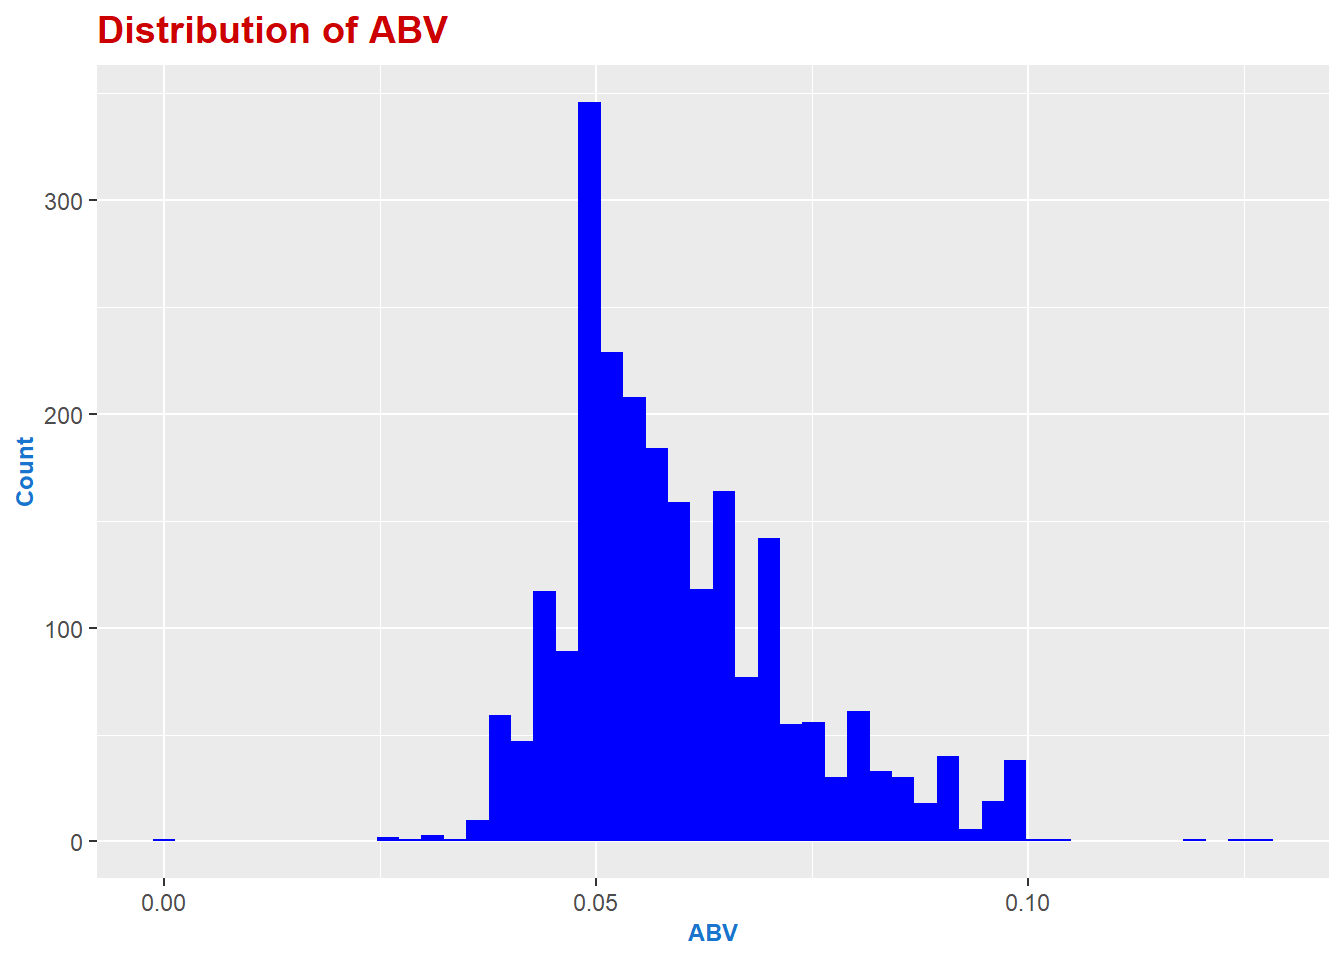
\includegraphics{Case-Study-Final_files/figure-latex/unnamed-chunk-9-1.pdf}

\begin{Shaded}
\begin{Highlighting}[]
\CommentTok{\#Boxplot}
\NormalTok{ABVclean}\SpecialCharTok{\%\textgreater{}\%}\FunctionTok{ggplot}\NormalTok{(}\FunctionTok{aes}\NormalTok{(}\AttributeTok{x=}\NormalTok{ABV))}\SpecialCharTok{+}
  \FunctionTok{geom\_boxplot}\NormalTok{(}\FunctionTok{aes}\NormalTok{(),}\AttributeTok{fill=}\StringTok{\textquotesingle{}red\textquotesingle{}}\NormalTok{)}\SpecialCharTok{+}
  \FunctionTok{ylab}\NormalTok{(}\StringTok{\textquotesingle{}ABV\textquotesingle{}}\NormalTok{)}\SpecialCharTok{+}
  \FunctionTok{ggtitle}\NormalTok{(}\StringTok{\textquotesingle{}Distribution of ABV\textquotesingle{}}\NormalTok{)}\SpecialCharTok{+}
  \FunctionTok{theme}\NormalTok{(}\AttributeTok{legend.position =} \StringTok{"bottom"}\NormalTok{,}
        \AttributeTok{legend.text =} \FunctionTok{element\_text}\NormalTok{(}\AttributeTok{size=}\DecValTok{7}\NormalTok{),}
        \AttributeTok{legend.title =} \FunctionTok{element\_text}\NormalTok{(}\AttributeTok{face=}\StringTok{"bold"}\NormalTok{, }\AttributeTok{color =} \StringTok{"black"}\NormalTok{, }\AttributeTok{size =} \DecValTok{8}\NormalTok{),}
        \AttributeTok{axis.text.y =} \FunctionTok{element\_blank}\NormalTok{(),}
        \AttributeTok{axis.title.y =} \FunctionTok{element\_blank}\NormalTok{(),}
        \AttributeTok{axis.ticks.y =} \FunctionTok{element\_blank}\NormalTok{(),}
        \AttributeTok{title =} \FunctionTok{element\_text}\NormalTok{(}\AttributeTok{face=}\StringTok{"bold"}\NormalTok{, }\AttributeTok{color =} \StringTok{"red3"}\NormalTok{, }\AttributeTok{size =} \DecValTok{12}\NormalTok{),}
        \AttributeTok{axis.title.x =} \FunctionTok{element\_text}\NormalTok{(}\AttributeTok{face=}\StringTok{"bold"}\NormalTok{, }\AttributeTok{color =} \StringTok{"dodgerblue3"}\NormalTok{, }\AttributeTok{size =} \DecValTok{9}\NormalTok{),)}
\end{Highlighting}
\end{Shaded}

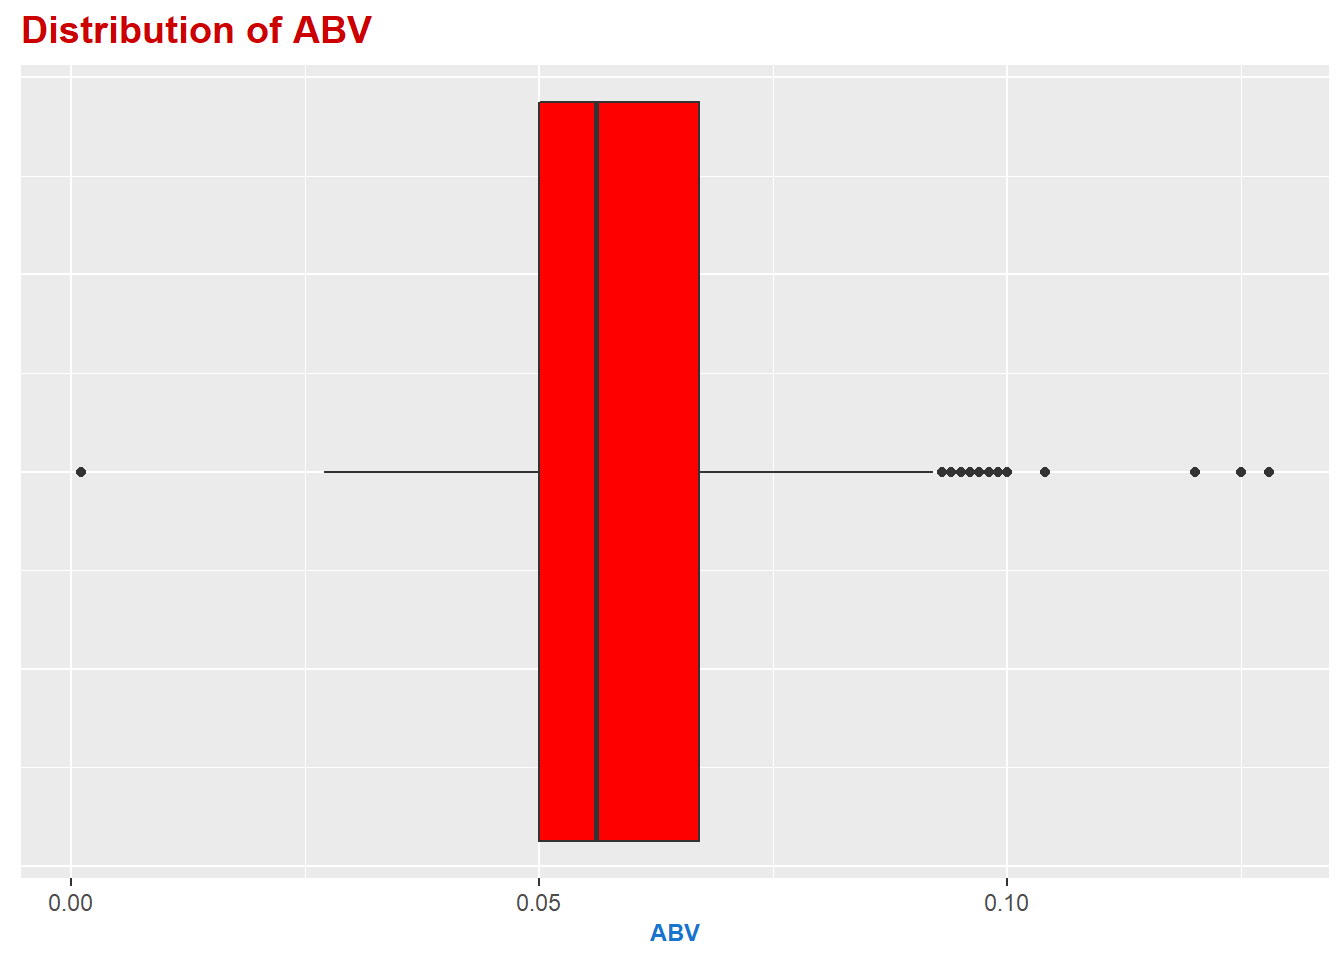
\includegraphics{Case-Study-Final_files/figure-latex/unnamed-chunk-9-2.pdf}

\begin{Shaded}
\begin{Highlighting}[]
\NormalTok{SummaryABV }\OtherTok{=} \FunctionTok{summary}\NormalTok{(ABVclean}\SpecialCharTok{$}\NormalTok{ABV)}

\NormalTok{SummaryABV}
\end{Highlighting}
\end{Shaded}

\begin{verbatim}
##    Min. 1st Qu.  Median    Mean 3rd Qu.    Max. 
## 0.00100 0.05000 0.05600 0.05977 0.06700 0.12800
\end{verbatim}

The first data table shows the summary statistics of ABV values if we
excluded all NA values for ABV and IBU. The histogram, boxplot and the
second data table account for all present ABV values. From histogram and
boxplot, we can see that the distribution of ABV's is right skewed. This
is confirmed by the second table in that the median is less than the
mean. The average ABV is 0.05977 with the lowest ABV at 0.001 and the
highest at 0.128. The interquartile range of the beers is between 0.05
and 0.067.

Question 7: Relationship between Bitterness of beer and its Alcohol
Content

\begin{Shaded}
\begin{Highlighting}[]
\CommentTok{\#How does the correlation between ABV and IBU change as either increase?}
\CommentTok{\#Scatter Plot ABV and IBU}

\CommentTok{\#Check correlation at lower ABV values}
\NormalTok{beerbreweries}\SpecialCharTok{\%\textgreater{}\%}\FunctionTok{filter}\NormalTok{(ABV}\SpecialCharTok{\textless{}}\FloatTok{0.0625}\NormalTok{)}\SpecialCharTok{\%\textgreater{}\%}
  \FunctionTok{ggplot}\NormalTok{(}\FunctionTok{aes}\NormalTok{(}\AttributeTok{x=}\NormalTok{ABV,}\AttributeTok{y=}\NormalTok{IBU))}\SpecialCharTok{+}
  \FunctionTok{geom\_point}\NormalTok{(}\FunctionTok{aes}\NormalTok{(),}\AttributeTok{color=}\StringTok{\textquotesingle{}blue\textquotesingle{}}\NormalTok{)}\SpecialCharTok{+}
  \FunctionTok{geom\_smooth}\NormalTok{(}\AttributeTok{method=}\StringTok{"lm"}\NormalTok{)}\SpecialCharTok{+}
  \FunctionTok{ggtitle}\NormalTok{(}\StringTok{\textquotesingle{}Bitterness vs Alcohol Content (ABV\textless{}0.0625)\textquotesingle{}}\NormalTok{)}\SpecialCharTok{+}
  \FunctionTok{xlab}\NormalTok{(}\StringTok{\textquotesingle{}Alcohol Content (ABV)\textquotesingle{}}\NormalTok{)}\SpecialCharTok{+}
  \FunctionTok{ylab}\NormalTok{(}\StringTok{\textquotesingle{}Bitterness (IBU)\textquotesingle{}}\NormalTok{)}\SpecialCharTok{+}
  \FunctionTok{theme}\NormalTok{(}\AttributeTok{title =} \FunctionTok{element\_text}\NormalTok{(}\AttributeTok{face=}\StringTok{"bold"}\NormalTok{, }\AttributeTok{color =} \StringTok{"red3"}\NormalTok{, }\AttributeTok{size =} \DecValTok{12}\NormalTok{),}
        \AttributeTok{axis.title.x =} \FunctionTok{element\_text}\NormalTok{(}\AttributeTok{face=}\StringTok{"bold"}\NormalTok{, }\AttributeTok{color =} \StringTok{"dodgerblue3"}\NormalTok{, }\AttributeTok{size =} \DecValTok{9}\NormalTok{),}
        \AttributeTok{axis.title.y =} \FunctionTok{element\_text}\NormalTok{(}\AttributeTok{face=}\StringTok{"bold"}\NormalTok{, }\AttributeTok{color =} \StringTok{"dodgerblue3"}\NormalTok{, }\AttributeTok{size =} \DecValTok{9}\NormalTok{))}
\end{Highlighting}
\end{Shaded}

\begin{verbatim}
## `geom_smooth()` using formula 'y ~ x'
\end{verbatim}

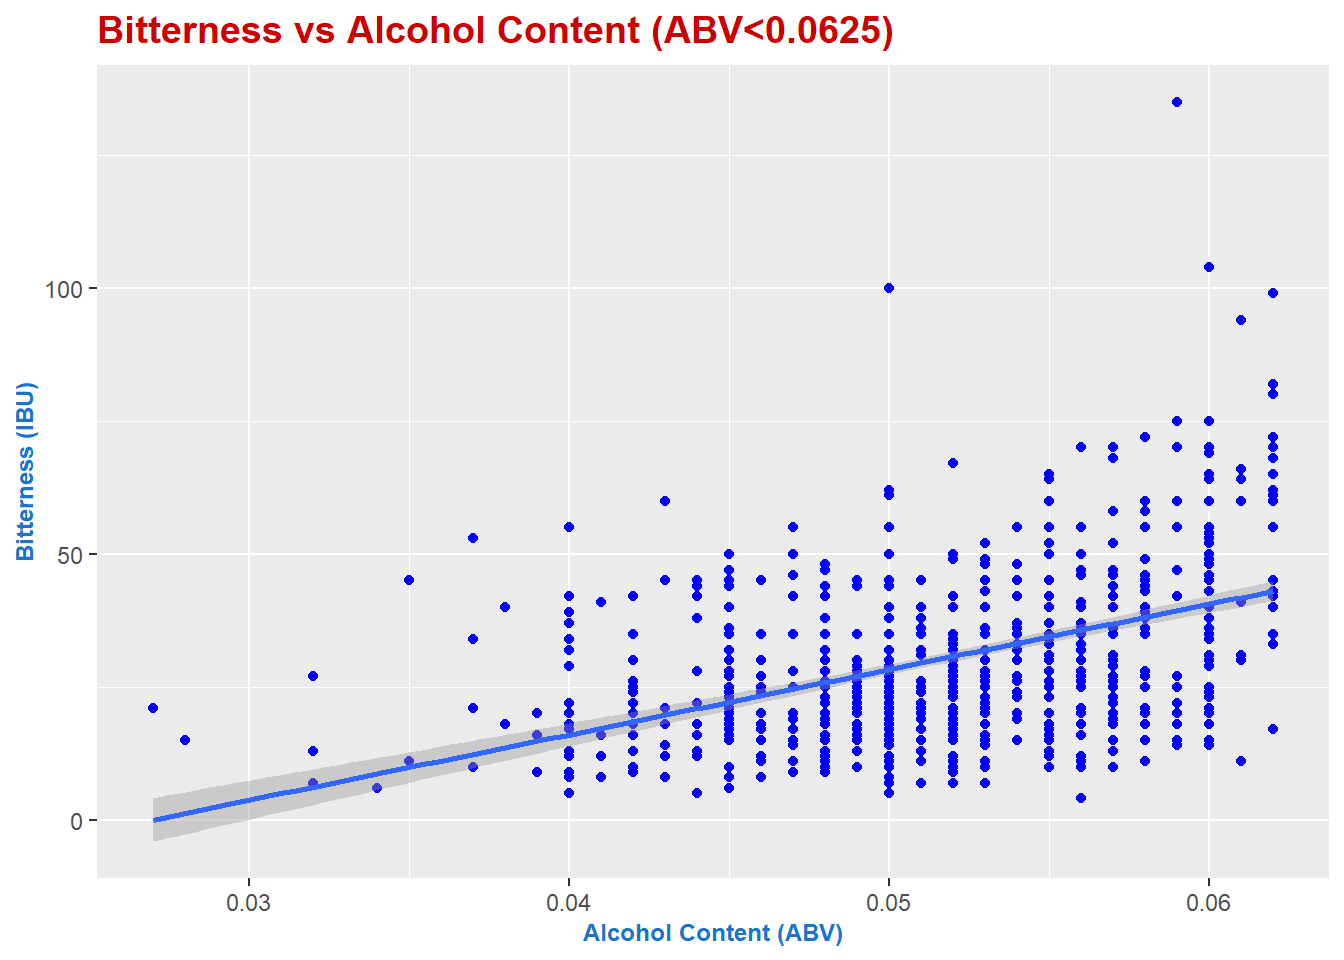
\includegraphics{Case-Study-Final_files/figure-latex/unnamed-chunk-10-1.pdf}

\begin{Shaded}
\begin{Highlighting}[]
\CommentTok{\#Find R\^{}2 at lower values}
\NormalTok{LowABV}\OtherTok{=}\FunctionTok{as.data.frame}\NormalTok{(beerbreweries}\SpecialCharTok{\%\textgreater{}\%}\FunctionTok{filter}\NormalTok{(ABV}\SpecialCharTok{\textless{}}\FloatTok{0.0625}\NormalTok{))}
\NormalTok{LmodLow}\OtherTok{=}\FunctionTok{lm}\NormalTok{(IBU}\SpecialCharTok{\textasciitilde{}}\NormalTok{ABV,LowABV)}
\FunctionTok{summary}\NormalTok{(LmodLow)}\CommentTok{\#r\^{}2=0.1971}
\end{Highlighting}
\end{Shaded}

\begin{verbatim}
## 
## Call:
## lm(formula = IBU ~ ABV, data = LowABV)
## 
## Residuals:
##     Min      1Q  Median      3Q     Max 
## -31.684 -10.226  -2.684   8.720  95.629 
## 
## Coefficients:
##             Estimate Std. Error t value Pr(>|t|)    
## (Intercept)  -33.138      4.291  -7.723    3e-14 ***
## ABV         1228.960     82.261  14.940   <2e-16 ***
## ---
## Signif. codes:  0 '***' 0.001 '**' 0.01 '*' 0.05 '.' 0.1 ' ' 1
## 
## Residual standard error: 14.93 on 909 degrees of freedom
## Multiple R-squared:  0.1971, Adjusted R-squared:  0.1963 
## F-statistic: 223.2 on 1 and 909 DF,  p-value: < 2.2e-16
\end{verbatim}

\begin{Shaded}
\begin{Highlighting}[]
\CommentTok{\#Check correlation at higher ABV values}
\NormalTok{beerbreweries}\SpecialCharTok{\%\textgreater{}\%}\FunctionTok{filter}\NormalTok{(ABV}\SpecialCharTok{\textgreater{}}\FloatTok{0.0625}\SpecialCharTok{\&}\NormalTok{ABV}\SpecialCharTok{\textless{}}\FloatTok{0.1}\NormalTok{)}\SpecialCharTok{\%\textgreater{}\%}
  \FunctionTok{ggplot}\NormalTok{(}\FunctionTok{aes}\NormalTok{(}\AttributeTok{x=}\NormalTok{ABV,}\AttributeTok{y=}\NormalTok{IBU))}\SpecialCharTok{+}
  \FunctionTok{geom\_point}\NormalTok{(}\FunctionTok{aes}\NormalTok{(),}\AttributeTok{color=}\StringTok{\textquotesingle{}blue\textquotesingle{}}\NormalTok{)}\SpecialCharTok{+}
  \FunctionTok{geom\_smooth}\NormalTok{(}\AttributeTok{method=}\StringTok{"lm"}\NormalTok{)}\SpecialCharTok{+}
  \FunctionTok{ggtitle}\NormalTok{(}\StringTok{\textquotesingle{}Bitterness vs Alcohol Content (ABV\textgreater{}0.0625)\textquotesingle{}}\NormalTok{)}\SpecialCharTok{+}
  \FunctionTok{xlab}\NormalTok{(}\StringTok{\textquotesingle{}Alcohol Content (ABV)\textquotesingle{}}\NormalTok{)}\SpecialCharTok{+}
  \FunctionTok{ylab}\NormalTok{(}\StringTok{\textquotesingle{}Bitterness (IBU)\textquotesingle{}}\NormalTok{)}\SpecialCharTok{+}
  \FunctionTok{theme}\NormalTok{(}\AttributeTok{title =} \FunctionTok{element\_text}\NormalTok{(}\AttributeTok{face=}\StringTok{"bold"}\NormalTok{, }\AttributeTok{color =} \StringTok{"red3"}\NormalTok{, }\AttributeTok{size =} \DecValTok{12}\NormalTok{),}
        \AttributeTok{axis.title.x =} \FunctionTok{element\_text}\NormalTok{(}\AttributeTok{face=}\StringTok{"bold"}\NormalTok{, }\AttributeTok{color =} \StringTok{"dodgerblue3"}\NormalTok{, }\AttributeTok{size =} \DecValTok{9}\NormalTok{),}
        \AttributeTok{axis.title.y =} \FunctionTok{element\_text}\NormalTok{(}\AttributeTok{face=}\StringTok{"bold"}\NormalTok{, }\AttributeTok{color =} \StringTok{"dodgerblue3"}\NormalTok{, }\AttributeTok{size =} \DecValTok{9}\NormalTok{))}
\end{Highlighting}
\end{Shaded}

\begin{verbatim}
## `geom_smooth()` using formula 'y ~ x'
\end{verbatim}

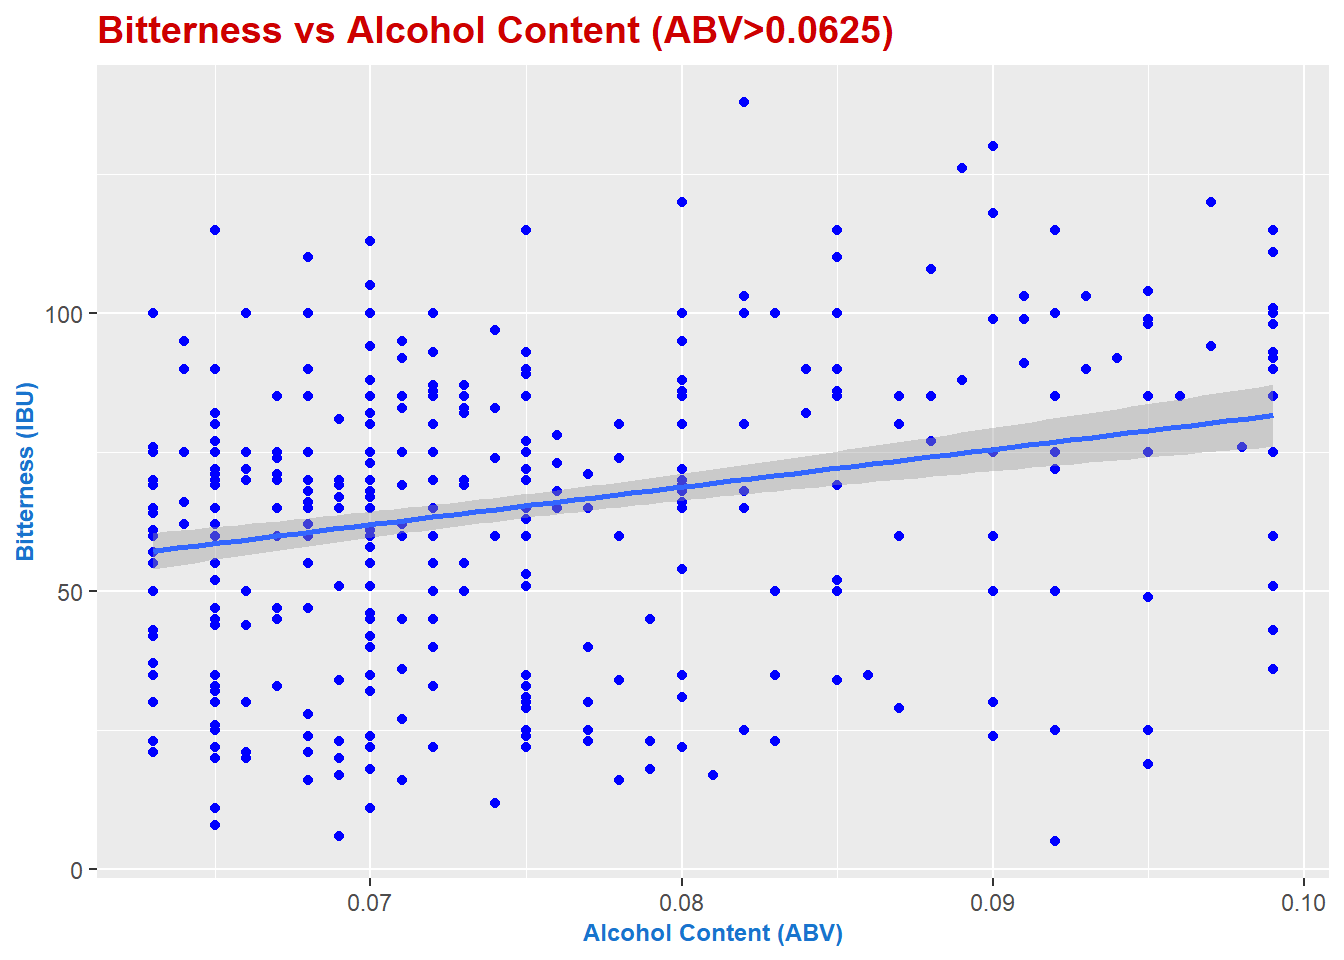
\includegraphics{Case-Study-Final_files/figure-latex/unnamed-chunk-10-2.pdf}

\begin{Shaded}
\begin{Highlighting}[]
\CommentTok{\#Find R\^{}2 at higher values}
\NormalTok{HighABV}\OtherTok{=}\FunctionTok{as.data.frame}\NormalTok{(beerbreweries}\SpecialCharTok{\%\textgreater{}\%}\FunctionTok{filter}\NormalTok{(ABV}\SpecialCharTok{\textgreater{}}\FloatTok{0.0625}\NormalTok{))}
\NormalTok{LmodHigh}\OtherTok{=}\FunctionTok{lm}\NormalTok{(IBU}\SpecialCharTok{\textasciitilde{}}\NormalTok{ABV,HighABV)}
\FunctionTok{summary}\NormalTok{(LmodHigh)}\CommentTok{\#r\^{}2=0.07411}
\end{Highlighting}
\end{Shaded}

\begin{verbatim}
## 
## Call:
## lm(formula = IBU ~ ABV, data = HighABV)
## 
## Residuals:
##     Min      1Q  Median      3Q     Max 
## -71.154 -14.866   6.087  14.507  68.255 
## 
## Coefficients:
##             Estimate Std. Error t value Pr(>|t|)    
## (Intercept)   17.193      7.721   2.227   0.0264 *  
## ABV          640.882    102.129   6.275 7.66e-10 ***
## ---
## Signif. codes:  0 '***' 0.001 '**' 0.01 '*' 0.05 '.' 0.1 ' ' 1
## 
## Residual standard error: 24.13 on 492 degrees of freedom
## Multiple R-squared:  0.07411,    Adjusted R-squared:  0.07222 
## F-statistic: 39.38 on 1 and 492 DF,  p-value: 7.664e-10
\end{verbatim}

\begin{Shaded}
\begin{Highlighting}[]
\CommentTok{\#Find overall r\^{}2}
\NormalTok{LmodTotal}\OtherTok{=}\FunctionTok{lm}\NormalTok{(IBU}\SpecialCharTok{\textasciitilde{}}\NormalTok{ABV,beerbreweries)}
\FunctionTok{summary}\NormalTok{(LmodTotal)}\CommentTok{\#r\^{}2=0.4497}
\end{Highlighting}
\end{Shaded}

\begin{verbatim}
## 
## Call:
## lm(formula = IBU ~ ABV, data = beerbreweries)
## 
## Residuals:
##     Min      1Q  Median      3Q     Max 
## -78.849 -11.977  -0.721  13.997  93.458 
## 
## Coefficients:
##             Estimate Std. Error t value Pr(>|t|)    
## (Intercept)  -34.099      2.326  -14.66   <2e-16 ***
## ABV         1282.037     37.860   33.86   <2e-16 ***
## ---
## Signif. codes:  0 '***' 0.001 '**' 0.01 '*' 0.05 '.' 0.1 ' ' 1
## 
## Residual standard error: 19.26 on 1403 degrees of freedom
## Multiple R-squared:  0.4497, Adjusted R-squared:  0.4493 
## F-statistic:  1147 on 1 and 1403 DF,  p-value: < 2.2e-16
\end{verbatim}

\begin{Shaded}
\begin{Highlighting}[]
\CommentTok{\#Both high and low lines on the same graph}
\NormalTok{HighLowAbv}\OtherTok{=}\FunctionTok{ifelse}\NormalTok{(beerbreweries}\SpecialCharTok{$}\NormalTok{ABV}\SpecialCharTok{\textgreater{}}\FloatTok{0.0625}\NormalTok{,}\StringTok{\textquotesingle{}High\textquotesingle{}}\NormalTok{,}\StringTok{\textquotesingle{}Low\textquotesingle{}}\NormalTok{)}
\NormalTok{beerbreweries}\SpecialCharTok{\%\textgreater{}\%}\FunctionTok{mutate}\NormalTok{(HighLowAbv)}\SpecialCharTok{\%\textgreater{}\%}
  \FunctionTok{ggplot}\NormalTok{(}\FunctionTok{aes}\NormalTok{(}\AttributeTok{x=}\NormalTok{ABV,}\AttributeTok{y=}\NormalTok{IBU))}\SpecialCharTok{+}
  \FunctionTok{geom\_point}\NormalTok{(}\FunctionTok{aes}\NormalTok{(),}\AttributeTok{col=}\FunctionTok{ifelse}\NormalTok{(beerbreweries}\SpecialCharTok{$}\NormalTok{ABV}\SpecialCharTok{\textgreater{}}\FloatTok{0.0625}\NormalTok{,}\StringTok{\textquotesingle{}blue\textquotesingle{}}\NormalTok{,}\StringTok{\textquotesingle{}red\textquotesingle{}}\NormalTok{))}\SpecialCharTok{+}
  \FunctionTok{geom\_smooth}\NormalTok{(}\AttributeTok{method=}\StringTok{\textquotesingle{}lm\textquotesingle{}}\NormalTok{,}\FunctionTok{aes}\NormalTok{(}\AttributeTok{col=}\NormalTok{HighLowAbv))}\SpecialCharTok{+}
  \FunctionTok{ggtitle}\NormalTok{(}\StringTok{\textquotesingle{}Bitterness vs Alcohol Content\textquotesingle{}}\NormalTok{)}\SpecialCharTok{+}
  \FunctionTok{xlab}\NormalTok{(}\StringTok{\textquotesingle{}Alcohol Content (ABV)\textquotesingle{}}\NormalTok{)}\SpecialCharTok{+}
  \FunctionTok{ylab}\NormalTok{(}\StringTok{\textquotesingle{}Bitterness (IBU)\textquotesingle{}}\NormalTok{)}\SpecialCharTok{+}
  \FunctionTok{theme}\NormalTok{(}\AttributeTok{title =} \FunctionTok{element\_text}\NormalTok{(}\AttributeTok{face=}\StringTok{"bold"}\NormalTok{, }\AttributeTok{color =} \StringTok{"red3"}\NormalTok{, }\AttributeTok{size =} \DecValTok{12}\NormalTok{),}
        \AttributeTok{axis.title.x =} \FunctionTok{element\_text}\NormalTok{(}\AttributeTok{face=}\StringTok{"bold"}\NormalTok{, }\AttributeTok{color =} \StringTok{"dodgerblue3"}\NormalTok{, }\AttributeTok{size =} \DecValTok{9}\NormalTok{),}
        \AttributeTok{axis.title.y =} \FunctionTok{element\_text}\NormalTok{(}\AttributeTok{face=}\StringTok{"bold"}\NormalTok{, }\AttributeTok{color =} \StringTok{"dodgerblue3"}\NormalTok{, }\AttributeTok{size =} \DecValTok{9}\NormalTok{),}
        \AttributeTok{legend.title=}\FunctionTok{element\_blank}\NormalTok{())}
\end{Highlighting}
\end{Shaded}

\begin{verbatim}
## `geom_smooth()` using formula 'y ~ x'
\end{verbatim}

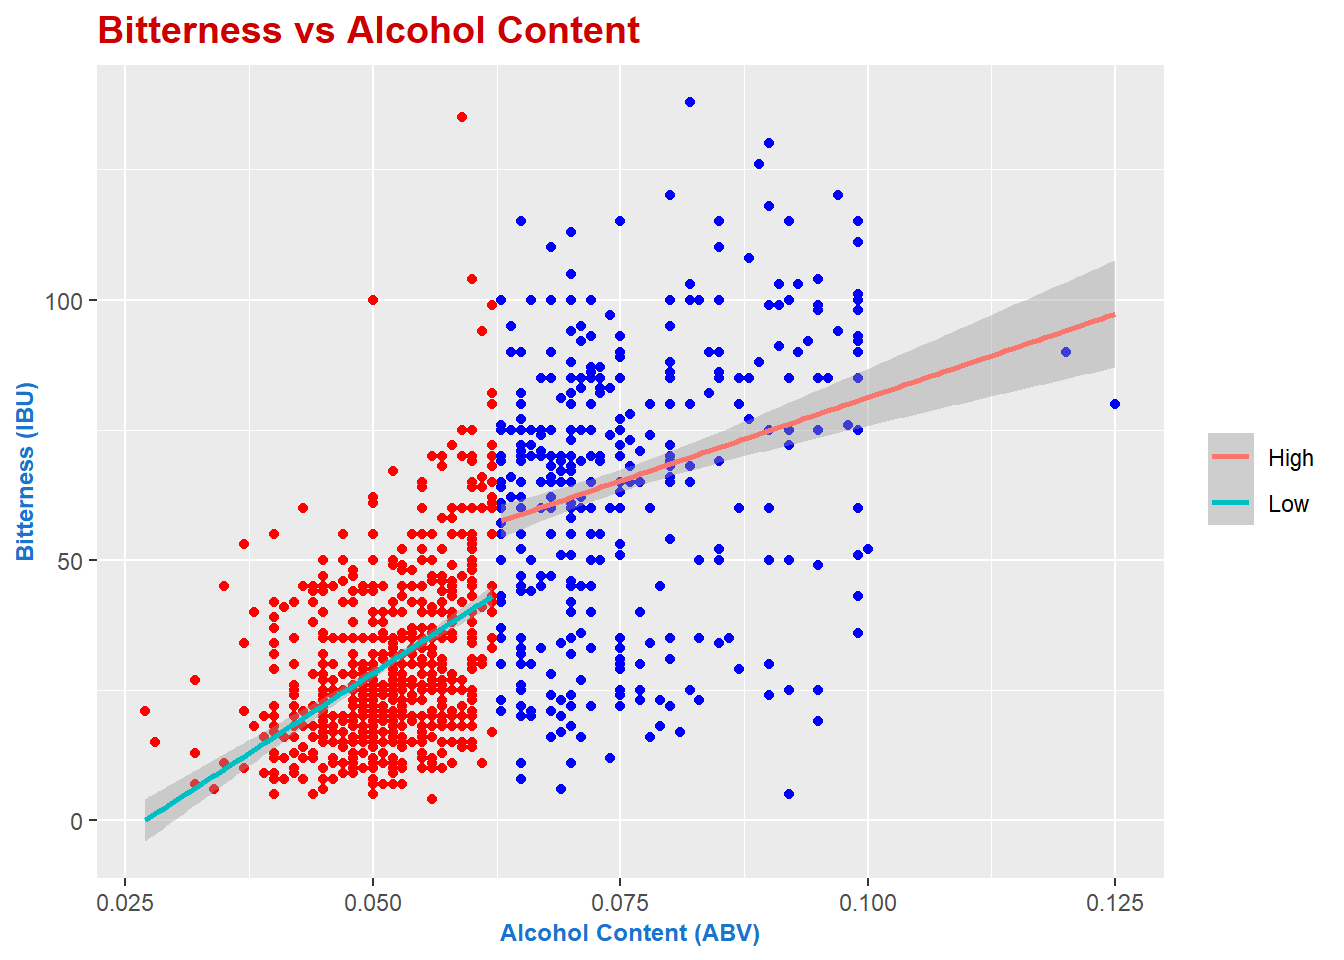
\includegraphics{Case-Study-Final_files/figure-latex/unnamed-chunk-10-3.pdf}
From the third graph, there appears to be a positive correlation between
alcohol content and bitterness. It is of note, that the correlation
appears weaker at the higher ABV and IBU. The percentage of estimated
variance in IBU is explained by changes in ABV is 44.97\%. Thus, we
divided the graph where the correlation between IBU and ABV increased
which was approximately at an ABV of 0.0625. The first scatterplot and
data table show the distribution for ABV and IBU for ABV values less
than 0.0625 where the least squares regression line has an R\^{}2 =
0.1971. The second scatterplot and data table show the distribution for
ABV and IBU for ABV values greater than 0.0625 where the least squares
regression line has an R\^{}2 = 0.07411. This supports our original
claim that the correlation appears weaker at the higher ABV and IBU.

Question 8: Predicting ALE or IPA based on ABV and IBU Content

\begin{Shaded}
\begin{Highlighting}[]
\CommentTok{\#Filter out beers that are either an Ale or an IPA}
\NormalTok{AleData}\OtherTok{=}\NormalTok{beers}\SpecialCharTok{\%\textgreater{}\%}\FunctionTok{filter}\NormalTok{((}\FunctionTok{grepl}\NormalTok{(}\StringTok{"(IPA)"}\NormalTok{,beers}\SpecialCharTok{$}\NormalTok{Style))}\SpecialCharTok{|}\NormalTok{(}\FunctionTok{grepl}\NormalTok{(}\StringTok{"(Ale)"}\NormalTok{,beers}\SpecialCharTok{$}\NormalTok{Name)))}


\CommentTok{\#Classify the drinks as either Ale or IPA}
\NormalTok{AleData}\SpecialCharTok{$}\NormalTok{IPAorALE}\OtherTok{=}\FunctionTok{ifelse}\NormalTok{(}\FunctionTok{grepl}\NormalTok{(}\StringTok{"IPA"}\NormalTok{,AleData}\SpecialCharTok{$}\NormalTok{Style),}\StringTok{"IPA"}\NormalTok{,}\StringTok{"Ale"}\NormalTok{)}
\NormalTok{AleClean}\OtherTok{=}\NormalTok{AleData}\SpecialCharTok{\%\textgreater{}\%}\FunctionTok{filter}\NormalTok{(}\SpecialCharTok{!}\NormalTok{(}\FunctionTok{is.na}\NormalTok{(IBU)}\SpecialCharTok{|}\FunctionTok{is.na}\NormalTok{(ABV)))}

\CommentTok{\#Set up Matrix to store Accuracy, Specificity,and Sensitivity values for the upcoming confusion matrix }
\NormalTok{iterations}\OtherTok{=}\DecValTok{500}
\NormalTok{numks}\OtherTok{=}\DecValTok{30}
\NormalTok{masterAcc}\OtherTok{=}\FunctionTok{matrix}\NormalTok{(}\AttributeTok{nrow=}\NormalTok{iterations,}\AttributeTok{ncol=}\NormalTok{numks)}
\NormalTok{masterSen}\OtherTok{=}\FunctionTok{matrix}\NormalTok{(}\AttributeTok{nrow=}\NormalTok{iterations,}\AttributeTok{ncol=}\NormalTok{numks)}
\NormalTok{masterSpec}\OtherTok{=}\FunctionTok{matrix}\NormalTok{(}\AttributeTok{nrow=}\NormalTok{iterations,}\AttributeTok{ncol=}\NormalTok{numks)}

\ControlFlowTok{for}\NormalTok{ (j }\ControlFlowTok{in} \DecValTok{1}\SpecialCharTok{:}\NormalTok{iterations)\{}
  \CommentTok{\#70{-}30 Training{-}Test Split}
  \FunctionTok{set.seed}\NormalTok{(}\FunctionTok{sample}\NormalTok{(}\DecValTok{1}\SpecialCharTok{:}\DecValTok{100000}\NormalTok{,}\DecValTok{1}\NormalTok{))}
\NormalTok{  trainInd}\OtherTok{=}\FunctionTok{sample}\NormalTok{(}\DecValTok{1}\SpecialCharTok{:}\FunctionTok{dim}\NormalTok{(AleClean)[}\DecValTok{1}\NormalTok{],}\FunctionTok{round}\NormalTok{(}\FloatTok{0.7}\SpecialCharTok{*}\FunctionTok{dim}\NormalTok{(AleClean)[}\DecValTok{1}\NormalTok{]))}
\NormalTok{  trainAle}\OtherTok{=}\NormalTok{AleClean[trainInd,]}
\NormalTok{  testAle}\OtherTok{=}\NormalTok{AleClean[}\SpecialCharTok{{-}}\NormalTok{trainInd,]}
  
  \ControlFlowTok{for}\NormalTok{(i }\ControlFlowTok{in} \DecValTok{1}\SpecialCharTok{:}\NormalTok{numks)\{}
    \CommentTok{\#k{-}NN to predict whether the drink is an IPA or an Ale}
\NormalTok{    AlePredictions}\OtherTok{=}\FunctionTok{knn}\NormalTok{(trainAle[,}\FunctionTok{c}\NormalTok{(}\StringTok{\textquotesingle{}ABV\textquotesingle{}}\NormalTok{,}\StringTok{\textquotesingle{}IBU\textquotesingle{}}\NormalTok{)],testAle[,}\FunctionTok{c}\NormalTok{(}\StringTok{\textquotesingle{}ABV\textquotesingle{}}\NormalTok{,}\StringTok{\textquotesingle{}IBU\textquotesingle{}}\NormalTok{)],trainAle}\SpecialCharTok{$}\NormalTok{IPAorALE,}\AttributeTok{k=}\NormalTok{i,}\AttributeTok{prob=}\ConstantTok{TRUE}\NormalTok{)}
\NormalTok{    AleTable}\OtherTok{=}\FunctionTok{table}\NormalTok{(AlePredictions,testAle}\SpecialCharTok{$}\NormalTok{IPAorALE)}
\NormalTok{    AleCM}\OtherTok{=}\FunctionTok{confusionMatrix}\NormalTok{(AleTable)}
\NormalTok{    masterAcc[j,i]}\OtherTok{=}\NormalTok{AleCM}\SpecialCharTok{$}\NormalTok{overall[}\DecValTok{1}\NormalTok{]}
\NormalTok{    masterSen[j,i]}\OtherTok{=}\NormalTok{AleCM}\SpecialCharTok{$}\NormalTok{byClass[}\DecValTok{1}\NormalTok{]}
\NormalTok{    masterSpec[j,i]}\OtherTok{=}\NormalTok{AleCM}\SpecialCharTok{$}\NormalTok{byClass[}\DecValTok{2}\NormalTok{]}
\NormalTok{  \}}
\NormalTok{\}}

\CommentTok{\#Collect the mean stats for each k{-}val}
\NormalTok{meanAcc}\OtherTok{=}\FunctionTok{colMeans}\NormalTok{(masterAcc)}
\NormalTok{meanSen}\OtherTok{=}\FunctionTok{colMeans}\NormalTok{(masterSen)}
\NormalTok{meanSpec}\OtherTok{=}\FunctionTok{colMeans}\NormalTok{(masterSpec)}

\CommentTok{\#Create dataframe with all stats}
\NormalTok{AleStats}\OtherTok{=}\FunctionTok{data.frame}\NormalTok{(}\AttributeTok{k=}\DecValTok{1}\SpecialCharTok{:}\DecValTok{30}\NormalTok{,}\AttributeTok{Mean\_Accuracy=}\NormalTok{meanAcc,}\AttributeTok{Mean\_Sensitivity=}\NormalTok{meanSen,}\AttributeTok{Mean\_Specificity=}\NormalTok{meanSpec,}\AttributeTok{Sum\_Stat=}\NormalTok{(meanSpec}\SpecialCharTok{+}\NormalTok{meanSen}\SpecialCharTok{+}\NormalTok{meanAcc))}

\CommentTok{\#Tune k{-}val based on all three stats}
\NormalTok{HighAleStats}\OtherTok{=}\NormalTok{AleStats}\SpecialCharTok{\%\textgreater{}\%}\FunctionTok{filter}\NormalTok{(Sum\_Stat}\SpecialCharTok{==}\FunctionTok{max}\NormalTok{(Sum\_Stat))}
\FunctionTok{formattable}\NormalTok{(HighAleStats)}
\end{Highlighting}
\end{Shaded}

k

Mean\_Accuracy

Mean\_Sensitivity

Mean\_Specificity

Sum\_Stat

4

0.8612837

0.8634406

0.860476

2.5852

\begin{Shaded}
\begin{Highlighting}[]
\CommentTok{\#k=4 seemed to give the best balance between accuracy, sensitivity, and specificity}
\CommentTok{\#I would prefer to use an odd number, but k=3,4, or 5 should provide good results regardless}

\CommentTok{\#70{-}30 Training{-}Test Split}
\FunctionTok{set.seed}\NormalTok{(}\FunctionTok{sample}\NormalTok{(}\DecValTok{1}\SpecialCharTok{:}\DecValTok{100000}\NormalTok{,}\DecValTok{1}\NormalTok{))}
\NormalTok{trainInd}\OtherTok{=}\FunctionTok{sample}\NormalTok{(}\DecValTok{1}\SpecialCharTok{:}\FunctionTok{dim}\NormalTok{(AleClean)[}\DecValTok{1}\NormalTok{],}\FunctionTok{round}\NormalTok{(}\FloatTok{0.7}\SpecialCharTok{*}\FunctionTok{dim}\NormalTok{(AleClean)[}\DecValTok{1}\NormalTok{]))}
\NormalTok{trainAle}\OtherTok{=}\NormalTok{AleClean[trainInd,]}
\NormalTok{testAle}\OtherTok{=}\NormalTok{AleClean[}\SpecialCharTok{{-}}\NormalTok{trainInd,]}

\CommentTok{\#3{-}NN to predict whether the drink is an IPA or an Ale}
\NormalTok{AlePredictions}\OtherTok{=}\FunctionTok{knn}\NormalTok{(trainAle[,}\FunctionTok{c}\NormalTok{(}\StringTok{\textquotesingle{}ABV\textquotesingle{}}\NormalTok{,}\StringTok{\textquotesingle{}IBU\textquotesingle{}}\NormalTok{)],testAle[,}\FunctionTok{c}\NormalTok{(}\StringTok{\textquotesingle{}ABV\textquotesingle{}}\NormalTok{,}\StringTok{\textquotesingle{}IBU\textquotesingle{}}\NormalTok{)],trainAle}\SpecialCharTok{$}\NormalTok{IPAorALE,}\AttributeTok{k=}\DecValTok{3}\NormalTok{,}\AttributeTok{prob=}\ConstantTok{TRUE}\NormalTok{)}
\NormalTok{AleTable}\OtherTok{=}\FunctionTok{table}\NormalTok{(AlePredictions,testAle}\SpecialCharTok{$}\NormalTok{IPAorALE)}
\FunctionTok{confusionMatrix}\NormalTok{(AleTable)}
\end{Highlighting}
\end{Shaded}

\begin{verbatim}
## Confusion Matrix and Statistics
## 
##               
## AlePredictions Ale IPA
##            Ale  85  15
##            IPA  14 101
##                                           
##                Accuracy : 0.8651          
##                  95% CI : (0.8121, 0.9078)
##     No Information Rate : 0.5395          
##     P-Value [Acc > NIR] : <2e-16          
##                                           
##                   Kappa : 0.7287          
##                                           
##  Mcnemar's Test P-Value : 1               
##                                           
##             Sensitivity : 0.8586          
##             Specificity : 0.8707          
##          Pos Pred Value : 0.8500          
##          Neg Pred Value : 0.8783          
##              Prevalence : 0.4605          
##          Detection Rate : 0.3953          
##    Detection Prevalence : 0.4651          
##       Balanced Accuracy : 0.8646          
##                                           
##        'Positive' Class : Ale             
## 
\end{verbatim}

\begin{Shaded}
\begin{Highlighting}[]
\CommentTok{\#Scatterplots of prediction and actual classifications}
\CommentTok{\#Scatterplot of actual classifications}
\NormalTok{testAle}\SpecialCharTok{\%\textgreater{}\%}\FunctionTok{ggplot}\NormalTok{(}\FunctionTok{aes}\NormalTok{(ABV,IBU,}\AttributeTok{color=}\NormalTok{IPAorALE))}\SpecialCharTok{+}
  \FunctionTok{geom\_point}\NormalTok{()}\SpecialCharTok{+}
  \FunctionTok{ggtitle}\NormalTok{(}\StringTok{\textquotesingle{}Bitterness vs Alcohol Content\textquotesingle{}}\NormalTok{)}\SpecialCharTok{+}
  \FunctionTok{xlab}\NormalTok{(}\StringTok{\textquotesingle{}Alcohol Content (ABV)\textquotesingle{}}\NormalTok{)}\SpecialCharTok{+}
  \FunctionTok{ylab}\NormalTok{(}\StringTok{\textquotesingle{}Bitterness (IBU)\textquotesingle{}}\NormalTok{)}\SpecialCharTok{+}
  \FunctionTok{theme}\NormalTok{(}\AttributeTok{title =} \FunctionTok{element\_text}\NormalTok{(}\AttributeTok{face=}\StringTok{"bold"}\NormalTok{, }\AttributeTok{color =} \StringTok{"red3"}\NormalTok{, }\AttributeTok{size =} \DecValTok{12}\NormalTok{),}
        \AttributeTok{legend.title =} \FunctionTok{element\_blank}\NormalTok{(),}
        \AttributeTok{axis.title.x =} \FunctionTok{element\_text}\NormalTok{(}\AttributeTok{face=}\StringTok{"bold"}\NormalTok{, }\AttributeTok{color =} \StringTok{"dodgerblue3"}\NormalTok{, }\AttributeTok{size =} \DecValTok{9}\NormalTok{),}
        \AttributeTok{axis.title.y =} \FunctionTok{element\_text}\NormalTok{(}\AttributeTok{face=}\StringTok{"bold"}\NormalTok{, }\AttributeTok{color =} \StringTok{"dodgerblue3"}\NormalTok{, }\AttributeTok{size =} \DecValTok{9}\NormalTok{))}
\end{Highlighting}
\end{Shaded}

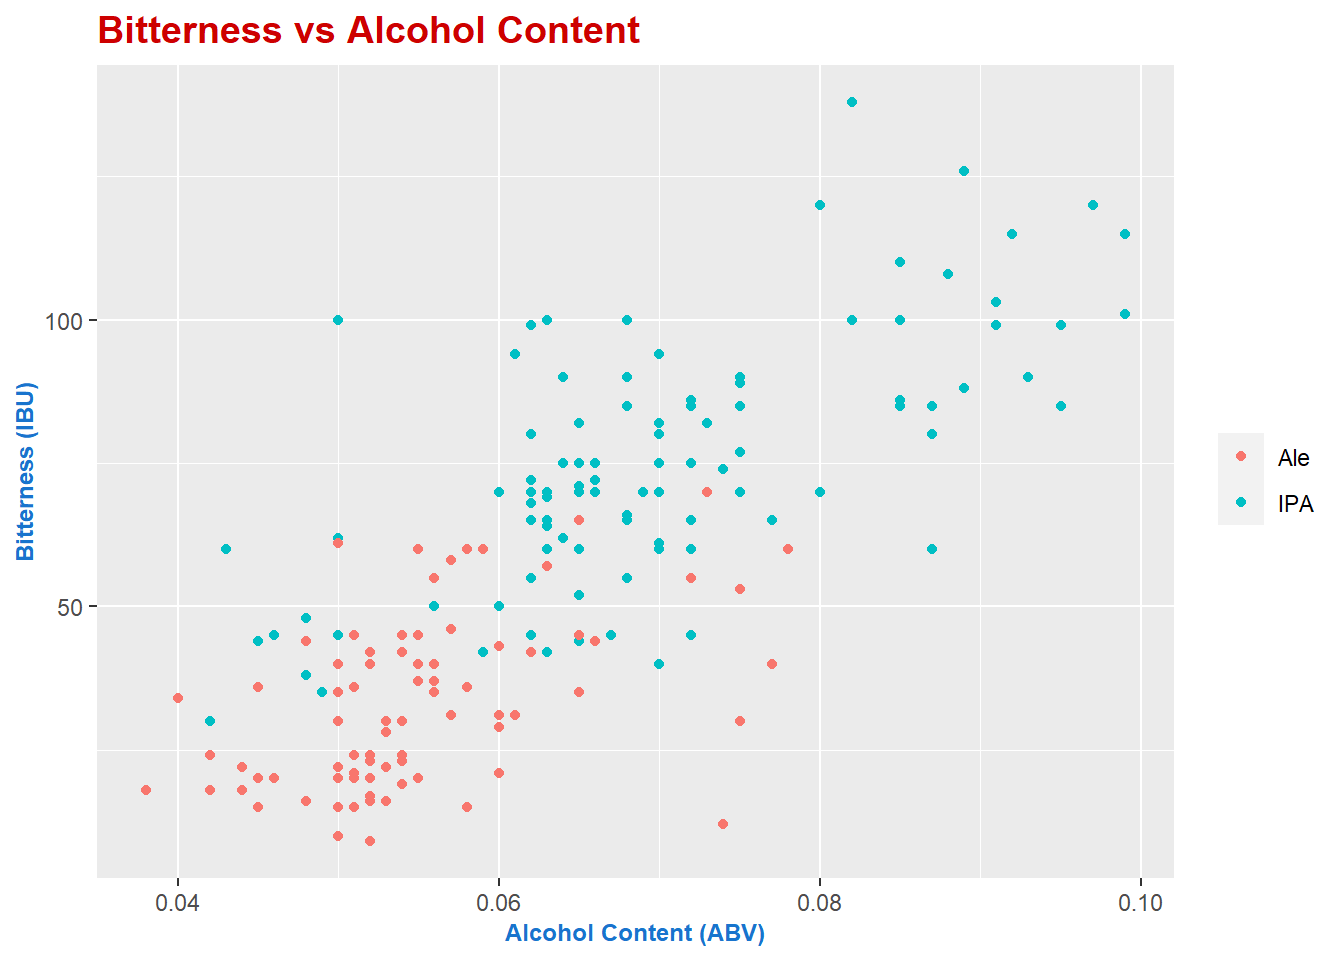
\includegraphics{Case-Study-Final_files/figure-latex/unnamed-chunk-11-1.pdf}
We tested a variety of k from 1 through 30 for our knn model over 500
iterations to find the optimal average accuracy, specificity and
sensitivity. The optimal k was found to be 4 but we decided to use k=3
since an odd k was more reasonable. We split the merged datasets into a
70-30 training and test set and found that the accuracy of this specific
model was 0.8837, the sensitivity was 0.8835, and the specificity was
0.8839.

\begin{Shaded}
\begin{Highlighting}[]
\CommentTok{\#Scatterplot of predicted classifications}
\NormalTok{testAle}\SpecialCharTok{\%\textgreater{}\%}\FunctionTok{mutate}\NormalTok{(AlePredictions)}\SpecialCharTok{\%\textgreater{}\%}
  \FunctionTok{ggplot}\NormalTok{(}\FunctionTok{aes}\NormalTok{(ABV,IBU,}\AttributeTok{color=}\NormalTok{AlePredictions))}\SpecialCharTok{+}
  \FunctionTok{geom\_point}\NormalTok{()}\SpecialCharTok{+}
  \FunctionTok{ggtitle}\NormalTok{(}\StringTok{\textquotesingle{}Bitterness vs Alcohol Content\textquotesingle{}}\NormalTok{)}\SpecialCharTok{+}
  \FunctionTok{xlab}\NormalTok{(}\StringTok{\textquotesingle{}Alcohol Content (ABV)\textquotesingle{}}\NormalTok{)}\SpecialCharTok{+}
  \FunctionTok{ylab}\NormalTok{(}\StringTok{\textquotesingle{}Bitterness (IBU)\textquotesingle{}}\NormalTok{)}\SpecialCharTok{+}
  \FunctionTok{theme}\NormalTok{(}\AttributeTok{title =} \FunctionTok{element\_text}\NormalTok{(}\AttributeTok{face=}\StringTok{"bold"}\NormalTok{, }\AttributeTok{color =} \StringTok{"red3"}\NormalTok{, }\AttributeTok{size =} \DecValTok{12}\NormalTok{),}
        \AttributeTok{legend.title=}\FunctionTok{element\_blank}\NormalTok{(),}
        \AttributeTok{axis.title.x =} \FunctionTok{element\_text}\NormalTok{(}\AttributeTok{face=}\StringTok{"bold"}\NormalTok{, }\AttributeTok{color =} \StringTok{"dodgerblue3"}\NormalTok{, }\AttributeTok{size =} \DecValTok{9}\NormalTok{),}
        \AttributeTok{axis.title.y =} \FunctionTok{element\_text}\NormalTok{(}\AttributeTok{face=}\StringTok{"bold"}\NormalTok{, }\AttributeTok{color =} \StringTok{"dodgerblue3"}\NormalTok{, }\AttributeTok{size =} \DecValTok{9}\NormalTok{))}
\end{Highlighting}
\end{Shaded}

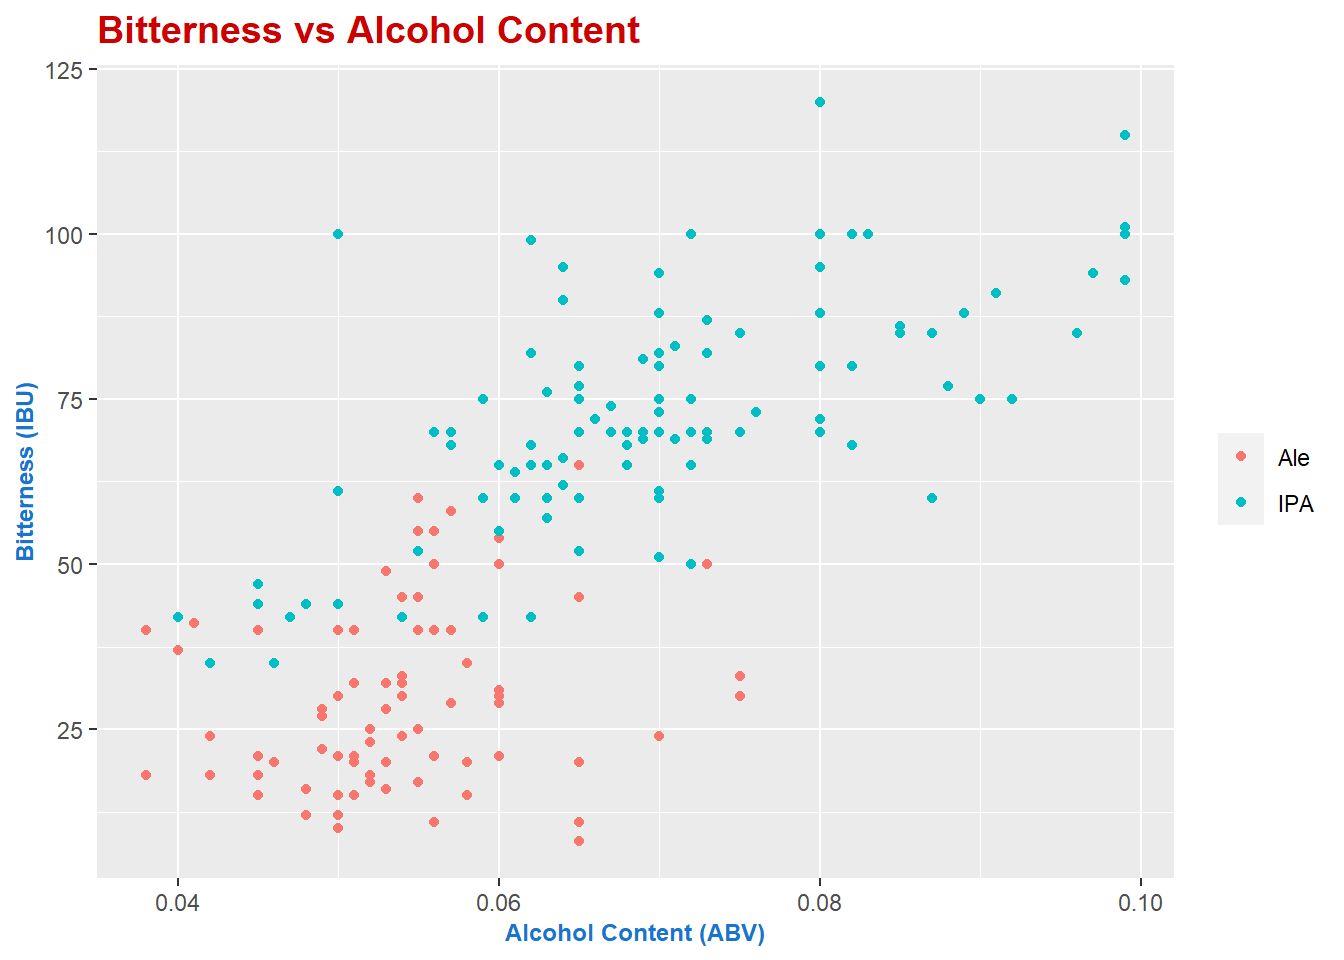
\includegraphics{Case-Study-Final_files/figure-latex/unnamed-chunk-12-1.pdf}

Above shows the scatterplot of the predicted classifications of either
Ale or IPA. It appears IBU and ABV levels is very accurate at explaining
whether or not a beverage is an IPA or an ale.

Question 9: Number of Beers per Brewery per State

We also found the number of beers produced per brewery for each state. A
bar graph is shown below. Washington DC was found to have the most beers
per brewery of all states.

\begin{Shaded}
\begin{Highlighting}[]
\NormalTok{beerbreweriesall }\OtherTok{=} \FunctionTok{merge}\NormalTok{(beers,breweries, }\AttributeTok{by.x=}\StringTok{"Brewery\_id"}\NormalTok{,}\AttributeTok{by.y=}\StringTok{"Brew\_ID"}\NormalTok{)}
\FunctionTok{colnames}\NormalTok{(beerbreweriesall)[}\DecValTok{1}\NormalTok{]}\OtherTok{=}\StringTok{\textquotesingle{}Brewery\_ID\textquotesingle{}}
\FunctionTok{colnames}\NormalTok{(beerbreweriesall)[}\DecValTok{2}\NormalTok{]}\OtherTok{=}\StringTok{\textquotesingle{}Beer\_Name\textquotesingle{}}
\FunctionTok{colnames}\NormalTok{(beerbreweriesall)[}\DecValTok{8}\NormalTok{]}\OtherTok{=}\StringTok{\textquotesingle{}Brewery\_Name\textquotesingle{}}

\NormalTok{beerbreweriesallsummarybystate }\OtherTok{=}\NormalTok{ beerbreweriesall}\SpecialCharTok{\%\textgreater{}\%}\FunctionTok{group\_by}\NormalTok{(State)}\SpecialCharTok{\%\textgreater{}\%}
  \FunctionTok{summarize}\NormalTok{(}\AttributeTok{Brewery\_Count=}\FunctionTok{n\_distinct}\NormalTok{(Brewery\_ID),}\AttributeTok{Beer\_Count=}\FunctionTok{n\_distinct}\NormalTok{(Beer\_ID))}
\NormalTok{beerbreweriesallsummarybystate}\SpecialCharTok{$}\NormalTok{Beer\_Per\_Brewery }\OtherTok{\textless{}{-}} \FunctionTok{round}\NormalTok{(beerbreweriesallsummarybystate}\SpecialCharTok{$}\NormalTok{Beer\_Count}\SpecialCharTok{/}\NormalTok{beerbreweriesallsummarybystate}\SpecialCharTok{$}\NormalTok{Brewery\_Count, }\AttributeTok{digit=}\DecValTok{1}\NormalTok{)}

\NormalTok{beerbreweriesallsummarybystate}\SpecialCharTok{\%\textgreater{}\%}
  \FunctionTok{ggplot}\NormalTok{(}\FunctionTok{aes}\NormalTok{(}\AttributeTok{x=}\FunctionTok{reorder}\NormalTok{(State,Beer\_Per\_Brewery),}\AttributeTok{y=}\NormalTok{Beer\_Per\_Brewery,}\AttributeTok{fill=}\NormalTok{Beer\_Per\_Brewery))}\SpecialCharTok{+}
  \FunctionTok{geom\_bar}\NormalTok{(}\AttributeTok{stat=}\StringTok{\textquotesingle{}identity\textquotesingle{}}\NormalTok{, }\AttributeTok{color =} \StringTok{"grey46"}\NormalTok{)}\SpecialCharTok{+}
  \FunctionTok{geom\_text}\NormalTok{(}\FunctionTok{aes}\NormalTok{(}\AttributeTok{label  =}\NormalTok{ Beer\_Per\_Brewery), }\AttributeTok{vjust =} \SpecialCharTok{{-}}\FloatTok{1.5}\NormalTok{, }\AttributeTok{size =} \FloatTok{2.2}\NormalTok{, }\AttributeTok{color =} \StringTok{"black"}\NormalTok{,}\AttributeTok{fontface =}  \StringTok{"bold"}\NormalTok{)}\SpecialCharTok{+}
  \FunctionTok{ylim}\NormalTok{(}\DecValTok{0}\NormalTok{,}\DecValTok{9}\NormalTok{)}\SpecialCharTok{+}
  \FunctionTok{ggtitle}\NormalTok{(}\StringTok{\textquotesingle{}Beer Produced per Brewery in State\textquotesingle{}}\NormalTok{)}\SpecialCharTok{+}
  \FunctionTok{xlab}\NormalTok{(}\StringTok{\textquotesingle{}State\textquotesingle{}}\NormalTok{)}\SpecialCharTok{+}
  \FunctionTok{ylab}\NormalTok{(}\StringTok{\textquotesingle{}Avg. Beer per Brewery\textquotesingle{}}\NormalTok{)}\SpecialCharTok{+}
  \FunctionTok{scale\_fill\_gradient2}\NormalTok{(}\AttributeTok{low =} \StringTok{"blue"}\NormalTok{, }\AttributeTok{mid =} \StringTok{"white"}\NormalTok{, }\AttributeTok{high =} \StringTok{"red4"}\NormalTok{, }
                       \AttributeTok{midpoint =} \DecValTok{4}\NormalTok{, }\AttributeTok{limits =} \FunctionTok{c}\NormalTok{(}\DecValTok{1}\NormalTok{,}\DecValTok{8}\NormalTok{), }
                       \AttributeTok{breaks=}\FunctionTok{c}\NormalTok{(}\DecValTok{1}\NormalTok{,}\DecValTok{2}\NormalTok{,}\DecValTok{3}\NormalTok{,}\DecValTok{4}\NormalTok{,}\DecValTok{5}\NormalTok{,}\DecValTok{6}\NormalTok{,}\DecValTok{7}\NormalTok{,}\DecValTok{8}\NormalTok{), }\AttributeTok{na.value =} \StringTok{"grey50"}\NormalTok{)}\SpecialCharTok{+}
  \FunctionTok{theme}\NormalTok{(}\AttributeTok{legend.position =} \StringTok{"none"}\NormalTok{,}
        \AttributeTok{title =} \FunctionTok{element\_text}\NormalTok{(}\AttributeTok{face=}\StringTok{"bold"}\NormalTok{, }\AttributeTok{color =} \StringTok{"midnightblue"}\NormalTok{, }\AttributeTok{size =} \DecValTok{12}\NormalTok{),}
        \AttributeTok{axis.text.y =} \FunctionTok{element\_blank}\NormalTok{(),}
        \AttributeTok{axis.title.y =} \FunctionTok{element\_blank}\NormalTok{(),}
        \AttributeTok{axis.ticks.y =} \FunctionTok{element\_blank}\NormalTok{(),}
        \AttributeTok{axis.text.x =} \FunctionTok{element\_text}\NormalTok{(}\AttributeTok{size =} \DecValTok{7}\NormalTok{),}
        \AttributeTok{axis.title.x =} \FunctionTok{element\_text}\NormalTok{(}\AttributeTok{face=}\StringTok{"bold"}\NormalTok{, }\AttributeTok{color =} \StringTok{"midnightblue"}\NormalTok{, }\AttributeTok{size =} \DecValTok{9}\NormalTok{))}
\end{Highlighting}
\end{Shaded}

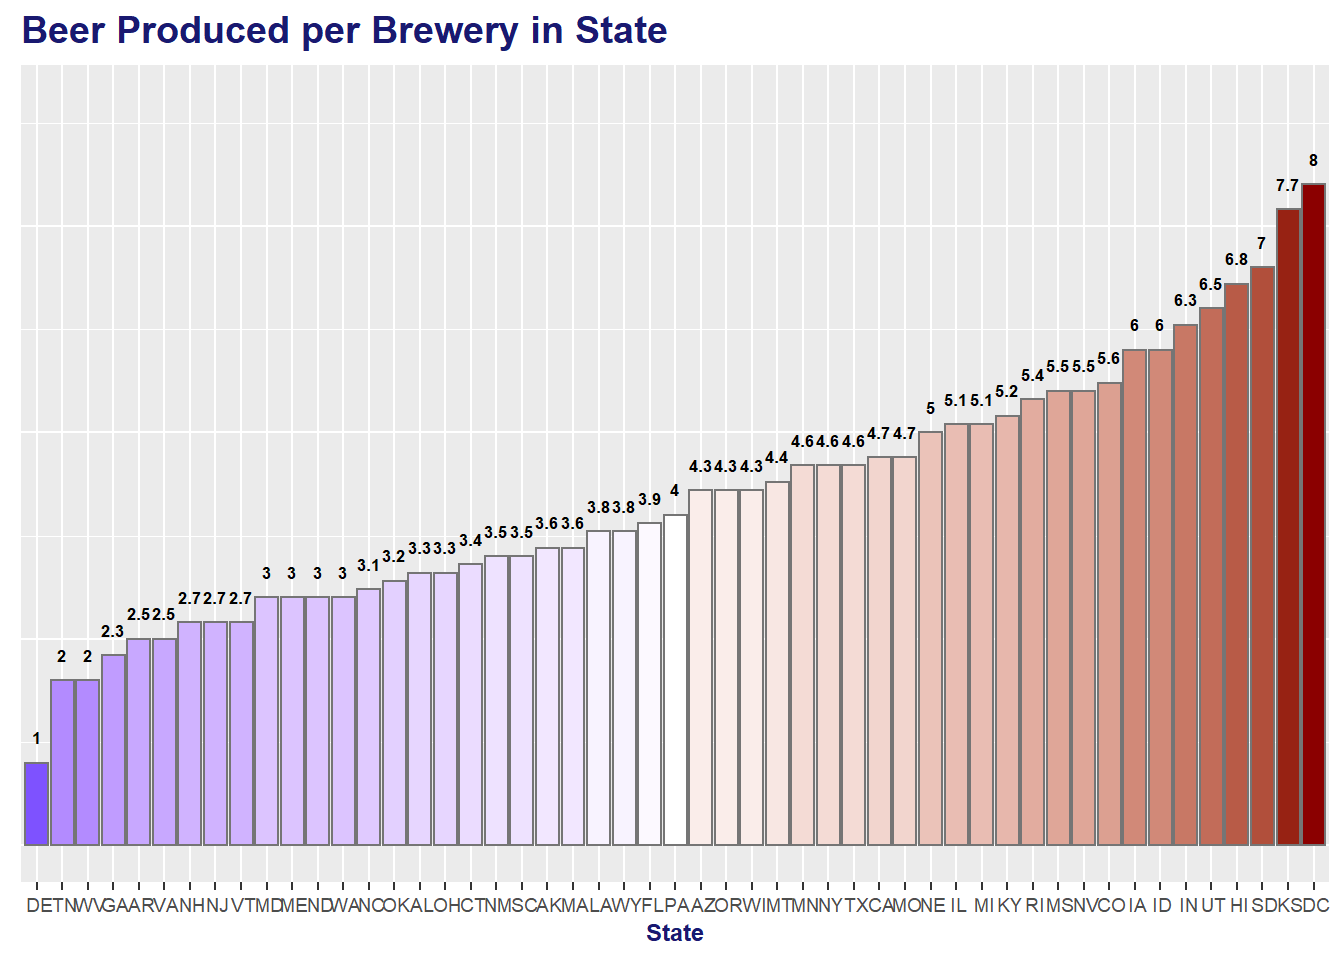
\includegraphics{Case-Study-Final_files/figure-latex/unnamed-chunk-13-1.pdf}

\begin{Shaded}
\begin{Highlighting}[]
\NormalTok{beerbreweriesallsummarybybrewery }\OtherTok{=}\NormalTok{ beerbreweriesall}\SpecialCharTok{\%\textgreater{}\%}\FunctionTok{group\_by}\NormalTok{(State,Brewery\_Name)}\SpecialCharTok{\%\textgreater{}\%}
  \FunctionTok{summarize}\NormalTok{(}\AttributeTok{Brewery\_Count=}\FunctionTok{n\_distinct}\NormalTok{(Brewery\_ID),}\AttributeTok{Beer\_Count=}\FunctionTok{n\_distinct}\NormalTok{(Beer\_ID))}
\end{Highlighting}
\end{Shaded}

\begin{verbatim}
## `summarise()` has grouped output by 'State'. You can override using the `.groups` argument.
\end{verbatim}

\begin{Shaded}
\begin{Highlighting}[]
\NormalTok{beerbreweriesallsummarybybrewery}\SpecialCharTok{$}\NormalTok{Beer\_Per\_Brewery }\OtherTok{\textless{}{-}} \FunctionTok{round}\NormalTok{(beerbreweriesallsummarybybrewery}\SpecialCharTok{$}\NormalTok{Beer\_Count}\SpecialCharTok{/}\NormalTok{beerbreweriesallsummarybybrewery}\SpecialCharTok{$}\NormalTok{Brewery\_Count, }\AttributeTok{digit=}\DecValTok{1}\NormalTok{)}

\NormalTok{Top\_Brewery}\OtherTok{=}\NormalTok{beerbreweriesallsummarybybrewery}\SpecialCharTok{\%\textgreater{}\%}\FunctionTok{filter}\NormalTok{(State}\SpecialCharTok{==}\StringTok{" DC"}\NormalTok{)}
\NormalTok{Top\_Brewery\_print}\OtherTok{=}\FunctionTok{data.frame}\NormalTok{(Top\_Brewery}\SpecialCharTok{$}\NormalTok{State,Top\_Brewery}\SpecialCharTok{$}\NormalTok{Brewery\_Name,Top\_Brewery}\SpecialCharTok{$}\NormalTok{Beer\_Count)}
\FunctionTok{names}\NormalTok{(Top\_Brewery\_print)}\OtherTok{=}\NormalTok{(}\FunctionTok{c}\NormalTok{(}\StringTok{\textquotesingle{}State\textquotesingle{}}\NormalTok{,}\StringTok{\textquotesingle{}Brewery Name\textquotesingle{}}\NormalTok{,}\StringTok{\textquotesingle{}Beer Count\textquotesingle{}}\NormalTok{))}
\FunctionTok{formattable}\NormalTok{(Top\_Brewery\_print)}
\end{Highlighting}
\end{Shaded}

State

Brewery Name

Beer Count

DC

DC Brau Brewing Company

8

From investigating the Beers and Breweries datasets, we found at least
one brewery in each state with CO, MI, and CA having at least 30.
Kentucky and Washington DC had the highest median ABV and Maine had the
highest median IBU. Colorado had the beer with the highest ABV
(Quadrupel (Quad)) whereas Oregon had the beer with the highest IBU
(IPA). The state with the highest number of beers per brewery was
Washington DC.

We found that ABV and IBU seemed to be positively correlated although
correlation seemed to weaken for higher values of ABV and IBU. Both
variables were approximately 88\% accurate in predicting whether a beer
was an Ale or an IPA. We appreciate the opportunity to work on this
analysis. If you have an questions, feel free to contact us at
\href{mailto:davidg@mail.smu.edu}{\nolinkurl{davidg@mail.smu.edu}},
\href{mailto:varung@mail.smu.edu}{\nolinkurl{varung@mail.smu.edu}}, or
\href{mailto:roslyns@mail.smu.edu}{\nolinkurl{roslyns@mail.smu.edu}}.

\end{document}
